\documentclass[11pt]{article}

\usepackage{natbib}
\bibliographystyle{abbrvnat}
\setcitestyle{authoryear,open={(},close={)}} 
\usepackage{multicol}
\usepackage{multirow}
\usepackage{booktabs}
\usepackage{caption}
\usepackage{amsmath}
\usepackage{longtable}
\usepackage{graphicx}
\usepackage{float}
\usepackage{bm}
\usepackage{graphics}
\usepackage{threeparttable}
\usepackage{amssymb}
\usepackage[margin=1in]{geometry}
\usepackage{setspace}
\usepackage{afterpage}
\doublespacing
\usepackage{subcaption}
\usepackage{subfig}
\usepackage{epigraph}
\usepackage{enumerate}
\usepackage{tabularx}
\usepackage{fancyhdr}
\usepackage{lscape}
\usepackage{mdframed}
\usepackage{mathtools}
\usepackage{array}
\usepackage{import}
\usepackage{fullpage}



\begin{document}
    \begin{titlepage}
    
    \title{Genetic Dilution erodes productivity: Exploring farmers' low adoption levels of improved maize in  Ethiopia}
% This second title is my preferred title at this point (28 Oct 2021). Open to other titles, but it shouldn't be longer than this one!

%     \author[1]{Oscar Barriga-Cabanillas}  
%     \author[2]{Cristina Chiarella}    
%     \author[2]{Juan Sebastian Correa}  	
%     \author[3]{Aleksandr Michuda}  

% 	\affil[1]{\small \emph{The World Bank}}
% 	\affil[2]{\small \emph{FAO}}
% 	\affil[3]{\small \emph{Assistant Research Professor at the Center for Data Science for Enterprise and Society, Cornell University}}
\author{%
 Aleksandr Michuda \footnote{Center for Data Science for Enterprise and Society, Cornell University}%
 \and Cristina Chiarella\footnote{Earth and Life Institute, UCLouvain, 1348 Louvain-la-Neuve, Belgium}%
 \and Oscar Barriga-Cabanillas\footnote{The World Bank}%
  \and Juan Sebastian Correa \footnote{Food and Agriculture Organization of the United Nations (FAO), 00153, Rome, Italy}%
  }

%   Assistant Research Professor at the 
	\date{\today}

    \clearpage\maketitle
	\thispagestyle{empty}
	\vspace*{-2em}
    \begin{center}\begin{abstract}
    \singlespacing
			\noindent  
			Despite large investments in  developing new  maize varieties, evidence shows that few farmers consistently adopt this new technology over time and that average effects mask considerable hetergeneity in impacts. Misclassification of seed is a crucial problem in these contexts, as non-classical measurement error can bias the impacts. We take a step further and study misclassification in the context of heterogeneous impacts to adoption. We use a three-year panel to estimate heterogeneous returns to adoption from self-reports of hybrid seed use and find peculiar results driven by bias due to the misclassification of seed. We exploit unique information on maize DNA-fingerprinting collected over the same areas in 2018. We find that misclassification in self-reported hybrid seed adoption mask heterogeneity in the actual quality of the genetic material of the seeds farmers categorized as improved varieties in the self-reported data. Positive returns to adoption are found for those farmers that use higher-purity germplasm, drought-tolerant maize, and newly released varieties. When we account for misclassification in our heterogeneity analysis, we find that the puzzle is resolved. Our findings point to the wide dispersion of older and genetically diluted varieties, for which poorer farmers may be paying a premium. The implications of our findings speak to the need for policies to better target context and geography, expand accessibility of improved seeds, and make higher yields varieties more inclusive.
			
			%Despite the large investments on creating better performing maize varieties, very few farmers consistently use them. We rely on four rounds of the ESS survey to answer this question. We find that relying on self reported use of hybrid seeds suggest there are negative returns to adoption. To reconcile this result, we use the information on genetic fingerprinting of seed available on the last ESS survey round to show that positive return for adoption appear only to exits for those farmers using seed with pure germoplast. We discuss the implications of our findings, showing that poorer farmers are the ones that consistently rely on second and third generation seeds, whose performance is debatable. 
        \end{abstract}\end{center}
        
        {\small \noindent\emph{JEL Classification}: O12, O13, O33, Q12, C13 \\
        	\emph{Keywords}: Improved maize, DNA-fingerprinting, Group Random Coefficient, Endogenous Switching Regression, Heterogeneous returns}

    \end{titlepage}
\maketitle
\newpage


%\begin{itemize}
%    \item Tim Weiss- hybrid subsidies
%    \item is there such a thing as traditional seeds?
%    \item Let's evaluate the effect of adoption in the context of Ethiopia
%    \item find ambiguous results, Why?
%    \item have access to DNA fingerprinting data
%    \item what do they say about adoption?
%    \item turns out that "adoption" isn't really a reliable concept/variable
%    \item most farmers are "adopting" under pretty conservative purity definitions
%    \item Let's see what happens with different varieties of seed, does adoption of that seed lead to positive yield effects?
%    \item can't use these methods but newer data has access to newer varieties where we're relatively more confident
%\end{itemize}

\section{Introduction}

%%% Why it is important
% Food security is a major challenge in many East African countries, and Ethiopia is no exception, having historically struggled to provide an adequate and reliable food supply \citep{Ramakrishna2002-hv, Jaleta2018-oj}. Since the drought of 1984, Ethiopia has become increasingly reliant on maize, and as of today, maize constitutes the most widespread crop in the country, with total area cultivated increasing and average yields almost doubling since 1990.\footnote{FAO statistics show the total area cultivated with Maize in 2019 is 25\% larger than the next most widespread crop (sorghum), and 27\% and 139\% larger than the next two following crops, wheat and barley, respectively.}\footnote{Improved security conditions and maize productivity contributed with an important decrease in undernourishment which fell from 47\% in 1990 to 14\% in 2018 (The World Bank, 2021). But despite these gains, food insecurity still affects more than half the population of Ethiopia. The country has also recently seen increases in food insecurity because of COVID-19, the conflict in Ethiopia’s Tigray region and the desert locust outbreak.} But despite this progress a large productivity gap persists between the African continent and the rest of the developing world.\footnote{From 2016 to the present, cereal crop yields in Sub-Saharan Africa have consistently been around 70-80\% lower than Europe or North America \citep{worldbankyield}.} The persistence of this gap is often attributed to different adoption rates of green revolution technologies, which include improved seeds. Evidence has shown that the adoption of improved seed leads to increases in agricultural yields \citep{Carter2014-fm}, food security \citep{Shiferaw2014-op}, and poverty reduction \citep{Minten2008-tj}.\footnote{Nevertheless, critics of green revolution technologies have also claimed that these technological packages have not been as profitable for many farmers in Africa as promised. Even the most successful of these countries, Ethiopia, is not on track to meet the goals of the Alliance for a Green Revolution for Africa (AGRA). This is due to high costs, and heavy dependence on subsidies \citep{Wise20}.} But in fact, only 13\% of maize farmers in Ethiopia have adopted improved seeds consistently between 2011 and 2015. A large percentage has adopted new varieties inconsistently, and the largest share of farmers (62\%) have not used improved seeds at all during the same period.  

%old version
% \footnote{FAO statistics show the total area cultivated with Maize in 2019 is 25\% larger than the next most widespread crop (sorghum), and 27\% and 139\% larger than the next two following crops, wheat and barley, respectively.} There was an upward trend in the total area cultivated with maize since 1990, with average yields almost doubling during this period.\footnote{Improved security conditions and maize productivity contributed with an important decrease in undernourishment which fell from 47\% in 1990 to 14\% in 2018 (The World Bank, 2021). But despite these positive gains in total area planted and average yields, food insecurity still affects more than half the population of Ethiopia.The country has also recently seen increases in food insecurity because of COVID-19, the conflict in Ethiopia’s Tigray region and the desert locust outbreak.} Despite progress a large productivity gap persists between the African continent and the rest of the developing world. From 2016 to the present, cereal crop yields in Sub-Saharan Africa have consistently been around 70-80\% lower than Europe or North America \citep{worldbankyield}. The persistence of this gap is often attributed to different adoption rates of green revolution technologies, which include improved seeds. Evidence has shown that the adoption of improved seed leads to increases in agricultural yields \citep{Carter2014-fm}, food security \citep{Shiferaw2014-op}, and poverty reduction \citep{Minten2008-tj}.\footnote{Nevertheless, critics of green revolution technologies have also claimed that these technological packages have not been as profitable for many farmers in Africa as promised. Even the most successful of these countries, Ethiopia, is not on track to meet the goals of the Alliance for a Green Revolution for Africa (AGRA). This is due to high costs, and heavy dependence on subsidies \citep{Wise20}.} 

% \begin{figure}[htp]
%     \centering
%     \caption{Maize: Total area harvested and average yields} \label{fig:maize_yields}
%     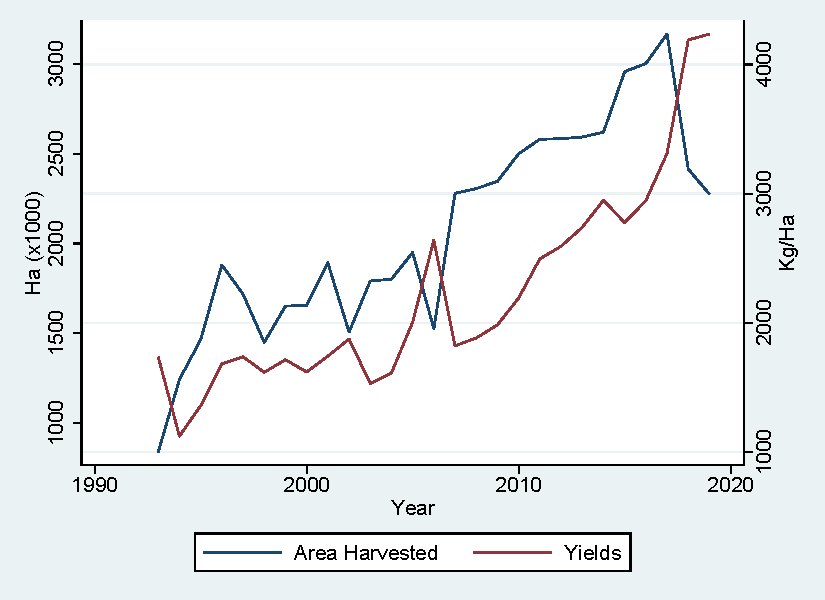
\includegraphics[width=.6\textwidth]{results/figures/Maize_yields.pdf}
%     \vspace*{-1em}
%     \begin{table}[H]
%         \centering
%         \begin{tabular}{p{0.6\textwidth}} 
%             \begin{tablenotes}[flushleft]
%                   \small
%                   \item Source: Authors' calculations using FAOSTAT data 
%                   \item Note: Yields are measured as the harvested production per ha for the area under cultivation
%             \end{tablenotes}
%         \end{tabular}
%     \end{table}       
% \end{figure}


%%%%% The puzzle 

Low adoption of hybrid seed, despite its benefits, has been a longstanding question in the study of agricultural technologies. Several answers have been proposed to explain such low adoption of improved varieties. These include lack of liquidity and other economic constraints \citep{Carter2014-fm}, growing conditions such as the type of soil, input use, and farmer characteristics \citep{Munshi2004-og}, imperfections in credit markets \citep{Croppenstedt2003-pq}, ambiguously defined property rights \citep{Place2000-el}, lack of commitment devices \citep{Duflo2009-iv}, high transportation costs that increase the cost of agricultural inputs \citep{Byerlee2013-qk}, and improved seed supply constraints \citep{Bird2020-nt}. An alternative mechanism for a lack of improvement has been the misclassification of seed and seed dilution (\citealt{wossen2022misperceiving}; \citealt{kosmowski2019varietal}). Net returns to improved seed is often lower than expected in the long term because a large percentage of farmers use diluted improved seed varieties, or ones that have been recycled over many generations (\citealt{euler2022because}; \citealt{wossen2019estimating}). Evidence suggests that yield improvement and disease resistance wanes over time \citep{Abate2015-rj}. Conversely, given the ubiquity of improved seed varieties over the course of decades of access in Ethiopia, some farmers may use improved seed without knowing it, leading to inferior yields than conventional seed due to a lack of the application of complementary inputs. 

Misclassification of improved seed and its implications for measuring productivity impacts has been a relatively new branch of study, with the advent of DNA fingerprinting data. For instance, \cite{wossen2019estimating} use DNA fingerprinting data to show that there is a 22\% bias in the productivity impact of improved cassava seed in Nigeria. In the context of hybrid seed adoption, however, there is evidence to suggest that productivity impacts of seed affect households heterogeneously \citep{Suri2011-oi}, and that average impacts to adoption may not be as informative. The observed effect of adoption may be low because households that would have a comparative advantage in adoption of improved seed are constrained by a lack of access to improved seed or infrastructure. Additionally, the non-classical measurement error introduced by misclassification can bias heterogeneity in ways that may attenuate or even reverse productivity impacts. This paper provides a way to account for misclassification of seed when additional, error-free data exists, such as DNA fingerprinting data. We estimate the comparative advantage of households directly using a Group Random Coefficients (GRC) Model and correct its heterogeneity estimates using misclassification rates from DNA fingerprinting data of the same plots \citep{Suri2011-oi, Tjernstrom_Emilia_Dalia_Ghanem_Oscar_Barriga_Cabanillas_Travis_J_Lybbert_Jeffrey_D_Michler_and_Aleksandr_Michuda2020-bc}. 


%%%% Let's evaluate the effect of adoption in the context of Ethiopia


%% Expand a bit on the methods
% We build on this literature by investigating improved maize seed adoption in Ethiopia. In particular, we implement two complementary estimation strategies to address both how heterogeneous returns drive the decision to use improved seed varieties, and the extent that the misclassification of varieties and genetic dilution affect the decision to adopt them by lowering their observed returns. First, we implement a Group Random Coefficients estimation, which builds on \cite{Suri2011-oi} and \cite{Tjernstrom_Emilia_Dalia_Ghanem_Oscar_Barriga_Cabanillas_Travis_J_Lybbert_Jeffrey_D_Michler_and_Aleksandr_Michuda2020-bc} using a General Method of Moments (GMM) estimator that allows us to test \textbf{ the assumptions made by \cite{Suri2011-oi}}, as well as provide more economically interpretable results. The advantage of our estimation strategy is that we do not rely on identification from a valid instrument. %\textbf{to assess XXXXXX}. %\footnote{Our estimation strategy is similar to \cite{Chamberlain1984-uk} \textbf{XXXXXX}.} 

Our results contribute to the literature on the drivers of low adoption rates of improved seed varieties. The consensus in this literature is that the success of improved varieties depends on a range of factors, and that the widespread adoption of  improved seeds is the result of complementary conditions and inputs that allow farmers to extract the full potential of these varieties. Specifically, extension services and on-farm field trials, seed variety characteristics and rainfall have been found to be crucial to the adoption of improved maize in Tanzania \citep{Kaliba2000-jh}. In the specific case of Ethiopia, labor, fertilizer use, farmers’ experience with extension packages, rainfall suitability and prices have been shown to increase the opportunity cost of not adopting improved wheat varieties \citep{Wale2006-bv}. Market access and the accessibility of extension services are also critical in the adoption of improved chickpea varieties in Ethiopia \citep{Verkaart2019-ol}. Other important determinants of heterogeneous effects include risk aversion \citep{Holden2016-vy}, farm size \citep{Ghimire2015-bd}, and credit constraints \citep{Simtowe2008-jn,Balana2020-hx}. We are the first to consider how heterogeneous impacts to seed adoption are affected by misclassification of seed.

% This implies that poorer farmers are paying a premium for genetically diluted hybrids, which has far-reaching policy implications about the need to foster a more inclusive strategy when making the best performing seeds available to all farmers


Our approach is divided into two parts. We start by using the first three survey rounds of the Ethiopian Socioeconomic Survey (ESS), which is a panel  covering  2011, 2013, and 2015. For each round, farmers self-reported on the seed variety they used (improved or traditional). To illustrate the effects of misclassification, we show the results of the GRC model for each ``adoption trajectory'' which is a sub-group characterized by the sequence of adoption choices made by the household. We find counter-intuitive results that seemingly show that households that adopt do not have a comparative advantage in adoption, or that households that adopt more often are less advantaged than those that adopt less. Returns to adoption are lowest for those that adopt more often.

Our second set of results use the fourth round of the ESS (conducted in 2018), which collected DNA fingerprints of harvested cropcuts in selected plots and compared its genetic material with a reference library of available varieties in Ethiopia, hence, providing a unique opportunity to understand why improved seed varieties seem not to increase returns when adopted. These data provides critical information not only about the seed types but also about their purity, sources, and their year of release. We exploit this uniquely rich information to compare returns of verifiable improved seed varieties against self-reported use of new, second generation or recycled varieties. For this, we leverage different purity thresholds (or degrees of no-contamination with other varieties), year of release, types of varieties, and their sources. Since many categorizations for DNA-fingerprinting exist, we implement an Endogenous Switching Regression (ESR) approach, to understand each categories' impact on adoption.\footnote{ESR is a standard estimation strategy to study the question of adoption with cross-sectional data (\citealt{Marenya2020-kb}, \citealt{Shiferaw2014-op}), given its capacity to account for unobserved heterogeneity in adoption.} The results of the ESR show negative effects of adopting improved seeds. But the comparison of different improved seed definitions using the DNA fingerprinting shows that when the definition of improved seed is based on greater purity of the germplasm (95\% of purity or more), returns to adoption becomes positive and significant. We obtain similar results when evaluating the specific effects of adopting drought-tolerant maize varieties, CGIAR or Exotic varieties, or more recently released varieties. 

Finally, to integrate our results together, we use the misclassification rates from the fourth round of the data and re-estimate the GRC results to be robust to misclassification (\citealt{michuda2021three}). We find that once we account for misclassification, heterogeneity in adoption becomes similar to other contexts: higher comparative advantage is associated with lower returns, pointing to significant barriers to adoption for those that would benefit the most from it. 


% A different branch of the literature provides an alternative explanation for the low adoption rates, focusing on heterogeneous potential returns to adoption \citep{Suri2011-oi}. This literature suggests that even if returns to adoption are high, farmers may fail to adopt if they face low comparative advantage to adoption. Other methods used in the literature fail to account for this heterogeneity, admitting only the presence of time-constant and/or time-varying unobserved heterogeneities (depending on the data structure) for identification purposes \citep{Kassie2018-xn,Falco2011-rt}. 

% We contribute to this literature by exploring heterogeneous comparative advantages to adoption in Ethiopia between 2011 to 2015. %, controlling for important drivers of adoption such as rainfall (found to be the main driver of heterogeneous effects for adopting agronomic packages \citealt{Marenya2020-kb}, \citealt{Katengeza2019-af}), labor and input use. 
% Our findings provide an alternative hypothesis to the puzzle of low maize adoption, namely that the wide dispersion of older generations and recycled improved seeds may be resulting in lower yields and altering farmers' input use. The null and negative effects that we see in the GRC results are actually stemming from misclassification in self-reported adoption status. This paper is the first to take seriously the bias that this can create when estimating the treatment effect of adoption, both in a homogeneous and heterogeneous setting. This also implies a methodological discovery when investigating hybrid seed adoption: the absence of a true control group to use for analysis. With more time and more genetic dilution, it becomes more likely that even those that do report hybrid use are still likely using some level of hybrid.


% A different branch of the literature provides an alternative explanation for the low adoption rates, focusing on heterogeneous potential returns to adoption \citep{Suri2011-oi}. This literature suggests that even if returns to adoption are high, farmers may fail to adopt if they face low comparative advantage to adoption. Other methods used in the literature fail to account for this heterogeneity, admitting only the presence of time-constant and/or time-varying unobserved heterogeneities (depending on the data structure) for identification purposes \citep{Kassie2018-xn,Falco2011-rt}.

The article continues as follows: in Section \ref{sec:data}, we describe the data used, the sample frame, general farmer and farm characteristics, and improved seed adoption levels. Section \ref{sec:strategy} presents the methodological details of our two estimation strategies. Section \ref{sec:results} shows the estimations results, Section \ref{sec:disc} discusses our findings in light of prior evidence, and Section \ref{sec:conclusion} presents the conclusion and implications of our analysis.


\section{Data}\label{sec:data}

This study uses the Ethiopia Socioeconomic Survey (ESS), part of the Agricultural Sample Survey (AgSS), a nationally representative survey designed to collect agricultural information for the major crops in Ethiopia. The survey is a joint effort of the the Central Statistics Agency of Ethiopia, the World Bank and CGIAR (Consortium of International Agricultural Research Centers) \citep{kosmowski2020shining}. The ESS contains four survey modules designed to obtain specific information about the different stages in the agricultural season. A post-planting questionnaire obtains information about the parcel, crop roster, seed roster and input use. A post-harvest questionnaire collects information about crop harvests by parcel (which includes cropcut measurements for selected plots), and crop disposition. These two instruments are complemented with a household and a community questionnaire, which obtain information on household characteristics, labor, land, expenditure, and community characteristics such as market prices and economic activities, respectively.

\subsection{The Three Round Panel and the Fourth Wave}

There were significant differences between the analysis carried out with the panel survey rounds (ESS 1-3) and the most recent survey round (ESS4). Most notably, the ESS4 is no longer a panel dataset made up of the households of ESS 1-3, but it includes important unique information on the DNA fingerprinting of seed type, which can be used to calculate misclassification rates. This is important information as the first three waves of ESS only included self-reported hybrid maize status. Since our estimation strategy to calculate returns to adoption requires a balanced panel dataset of maize growers, our main analysis includes the first three waves of the ESS. We use the fourth wave to provide further light on the low levels of returns from adoption we find in the first three ESS rounds, and to explore the impact of specific types of improved seeds.

Figure \ref{map:regions} shows the spatial distribution of the locations of the households in the study. These are households that grow either improved or conventional maize and that are observed for the three rounds of the survey. Most households come from the northwest region of Amhara, Tigray and Oromiya which is consistent with where maize is mostly grown in Ethiopia \citep{Abate2015-rj}.

\begin{figure}[H]
    \centering
    \caption{Spatial Distribution of Households Surveyed}\label{map:regions}
    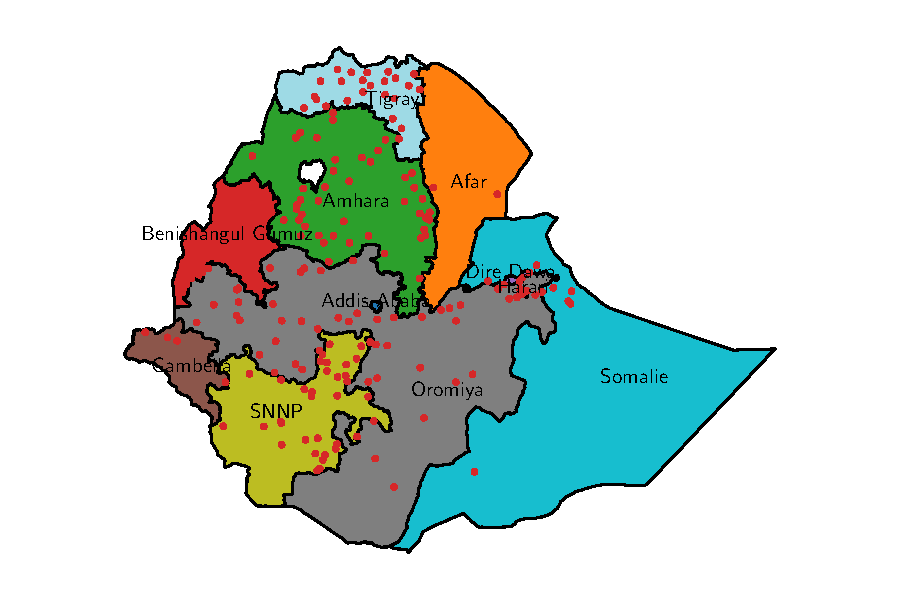
\includegraphics[width=.7\textwidth]{results/figures/map_hhids.pdf}
    \vspace*{-1em}
    \begin{table}[H]
        \centering
        \begin{tabular}{p{0.6\textwidth}} 
            \begin{tablenotes}
                  \small
                  \item Note: Red markers denote the locations of households. Coordinates are slightly modified and repeated for confidential reasons.
            \end{tablenotes}
        \end{tabular}
    \end{table}  
\end{figure}

Table \ref{tbl:summary} shows a set of summary statistics for the sample. The mean parcel size for a household is about 0.15 Ha, with a maximum size of less than 3.7 Ha. Harvest labor is disproportionately skewed to family participation with around 20 days of harvest labor being conducted by family members and only about 2 days for hired labor. This is indicative of either malfunctioning labor markets, income constraints or high supervision costs. The distances to some key areas are also highlighted in Table \ref{tbl:summary}. On average, households are around 13 kilometers away from an asphalt road and almost 60 kilometers away from the nearest market. This makes both the purchase of improved seed and the marketing of yields subject to transportation costs and a difficult enterprise. Fertilizer costs are on average 8,350 Birr ($\thicksim$178 USD), with a large amount of the sample not using fertilizer at all. This is particularly important in the context of improved maize seed use as these technologies are intensive in external inputs, such as chemical fertilizers and irrigation, to be effective. Only 5\% of the sample irrigates their crops making households susceptible to weather shocks.


\afterpage{{\footnotesize\tabcolsep=1pt  % hold it local
    \begin{table}
\centering
\caption{Summary Statistics for Households}
\label{tbl:summary}
\begin{tabular}{lllll}
\toprule
                             & Wave &       1.0 &       2.0 &       3.0 \\
\midrule
Parcel Size & N &  1,116.00 &  1,116.00 &  1,116.00 \\
                             & Mean &      0.31 &      0.32 &      0.30 \\
                             & Std. Dev. &      0.36 &      0.39 &      0.35 \\
Household Labor for Harvest (Days) & N &  1,116.00 &  1,116.00 &  1,116.00 \\
                             & Mean &     45.51 &     38.29 &     36.33 \\
                             & Std. Dev. &     71.11 &     54.58 &     46.56 \\
Hired Labor for Harvest (Days) & N &  1,116.00 &  1,116.00 &  1,116.00 \\
                             & Mean &      4.27 &      3.38 &      4.89 \\
                             & Std. Dev. &     25.93 &     17.08 &     54.11 \\
Age of Household Head & N &  1,106.00 &  1,086.00 &  1,102.00 \\
                             & Mean &     43.85 &     45.91 &     48.23 \\
                             & Std. Dev. &     14.31 &     14.17 &     14.33 \\
Sex of Household Head & N &  1,109.00 &  1,114.00 &  1,108.00 \\
                             & Mean &      1.15 &      1.15 &      1.16 \\
                             & Std. Dev. &      0.36 &      0.36 &      0.36 \\
Years of Education of Household Head & N &  1,106.00 &  1,085.00 &  1,102.00 \\
                             & Mean &      1.46 &      1.56 &      1.64 \\
                             & Std. Dev. &      2.71 &      2.77 &      2.92 \\
Total Rainfall (mm) & N &  1,113.00 &  1,088.00 &  1,106.00 \\
                             & Mean &    899.23 &    953.98 &    943.03 \\
                             & Std. Dev. &    240.43 &    237.46 &    267.07 \\
Does Household have Title to land? & N &  1,113.00 &  1,088.00 &  1,106.00 \\
                             & Mean &      0.43 &      0.52 &      0.61 \\
                             & Std. Dev. &      0.50 &      0.50 &      0.49 \\
Crop Cut Dry Yield (kg/ha) & N &  1,105.00 &  1,103.00 &  1,103.00 \\
                             & Mean &     86.51 &    251.69 &    438.42 \\
                             & Std. Dev. &    200.25 &    532.17 &    786.49 \\
Self-reported Yields (kg/ha) & N &  1,043.00 &  1,075.00 &  1,064.00 \\
                             & Mean &    187.18 &  1,314.04 &  1,224.65 \\
                             & Std. Dev. &    435.03 &  1,157.66 &  1,105.53 \\
\bottomrule
\multicolumn{6}{l}{Note: Parcel size, yield and distance variables winsorized at the 1\% level.}
\end{tabular}
\end{table}

    \vspace*{-4em}
    \begin{table}[H]
        \centering
        \begin{tabular}{p{0.7\textwidth}} 
            \begin{tablenotes}
                  \small
                  \item Note: Author's calculations using ESS. Maize farmers only.
            \end{tablenotes}
        \end{tabular}
    \end{table}  
    \newpage
}}

The ESS has both self-reported and crop cut yields available. This provides two sources of yield information, although self-reported yields seem to be overly large compared to either fresh or dried crop cut yields. Self-reported yields are both more susceptible to behavioral biases, but also to confusion caused by differences in assumed units. In general, though, the sample with available cropcut yields cuts down the available sample significantly, given that cropcuts were only collected for a subsample of randomly selected households.


\subsection{Improved Seeds}

A seed is considered “improved” in Ethiopia if it was tested by breeders and evaluated to be superior to existing varieties  (\citealp{MoA13}; \citealp{kosmowski2020shining}). In Ethiopia, the government controls most of the seed system, with local agricultural offices or extension agents assessing the demands of different varieties. The MoA decides the seed quantities to be produced, and actors such as regional seed enterprises, seed companies, seed unions, are involved in the production of certified seeds, which are later distributed by seed producer cooperatives (SPCs).\footnote{They account for 37\% of the total distribution in the country (\citealp{kosmowski2020shining}).} An improved seed can be obtained directly from such distribution centers (which would distribute a first generation seed), however it is often the case that seeds cultivated from second or later generations from the originally bred seed are also exchanged between farmers. In the survey, farmers are asked to report whether the variety they used was a first-generation improved seed, second generation, recycled, or a traditional variety. When buying seeds, farmers might be able to identify the variety they are looking for, but it is unlikely that they would be aware of the source. 

Fifty four varieties have been released in Ethiopia since 1990.\footnote{Out of which seven were released between 1990 to 1999, 29 between 2000 to 2009, and 18 between 2010 to 2019.} Thirty four such varieties contain International Maize and Wheat Improvement Center (CIMMYT) germplasm, out of which, 10 Drought-tolerant maize varieties (DTMZ) and 8 Quality protein maize (QPM) were released (most of these between 2010 to 2019). Besides the CIMMYT-related germplasm, ten are open-pollinated varieties (OPVs) and 25 are hybrid (\citealp{kosmowski2020shining}).

The fourth wave of the ESS introduced DNA fingerprinting of barley, maize, and sorghum for the first time. The collection of cropcuts for crop yield estimation facilitated the process for DNA fingerprinting. For the cropcuts, a four square meter quadrant was randomly selected in each plot, and total production harvested from the quadrant was weighed (both when freshly harvested and when dried). The DNA material was extracted from samples from the dried cropcuts, and were then matched with the genetic material of the maize DNA reference library for Ethiopia, obtained from a CIMMYT and Ethiopian Institute of Agricultural Research (EIAR) project. The collection of DNA samples focused on eight regions. In each enumeration area (EA) of these regions, a random sample of plots was selected, with a maximum of 10 fields for each crop. As a result, 505 plots were selected for DNA fingerprinting, corresponding to 447 households. 

The DNA fingerprinting process matched the genetic material of each sampled harvest with that of the reference library. The resulting matching process returns the name of the crop variety matched, its germplasm origin or their pedigree (whether they are a CIMMYT line, EIAR,  International Institute of Tropical Agriculture (IITA) or private), the breeder or maintainer, and the year of their release (which could be indicative of the number of generations a seed had been cultivated), as well as the genetic purity of the sample (the degree of non-contamination with other genetic varieties). It also informs whether the harvested seeds are open-pollinated varieties (OPVs) or hybrids; drought-tolerant maize varieties (DMTZ) or quality protein maize (QPM). This rich information about seed varieties provides a unique opportunity to further understand impacts differentiated by type of seed, degree of purity, year of release or source. Figure \ref{fig:adoption_r4} shows adoption rates in the fourth round for improved varieties, using the above characteristics as different definitions.

We find that 38\% of households self-report adopting a “new” improved variety (SR2 in Figure \ref{fig:adoption_r4}), and 43\% report adopting a “new”, “second generation” or “recycled” improved variety (SR1). Considering a household as adopter if the household planted an improved variety in at least one of their plots, leads to classifying all households where a DNA sample was obtained as users of improved seed variety, a result that holds when the purity threshold of 70\% (DNA 70) is used. It is only when using purity thresholds of 90 and 95\% (DNA 90, DNA 95 in Figure \ref{fig:adoption_r4}, respectively), that adoption rates of improved varieties change to 91 and 54\% of sampled households, respectively.\footnote{We also find that 62\% of households adopted a hybrid variety, compared to 38\% that adopted an open-pollinated variety, and 15\% of households adopted a drought-tolerant maize variety, while 63\% of households that adopted an improved variety use a CGIAR-derived germplasm, and 79\% use an exotic germplasm.} Finally, 64\% of households adopted a variety that was released in the year 2000 or after, and 24\% adopted a variety that was adopted in the year 2010 or after. These ratios are in line with prior findings (\citealp{Zeng15}).

\begin{figure}[htpb]
    \centering
    \caption{Adoption rates of improved varieties in 2018 (by self-report, purity level, crop type, source and year of release)}\label{fig:adoption_r4}
    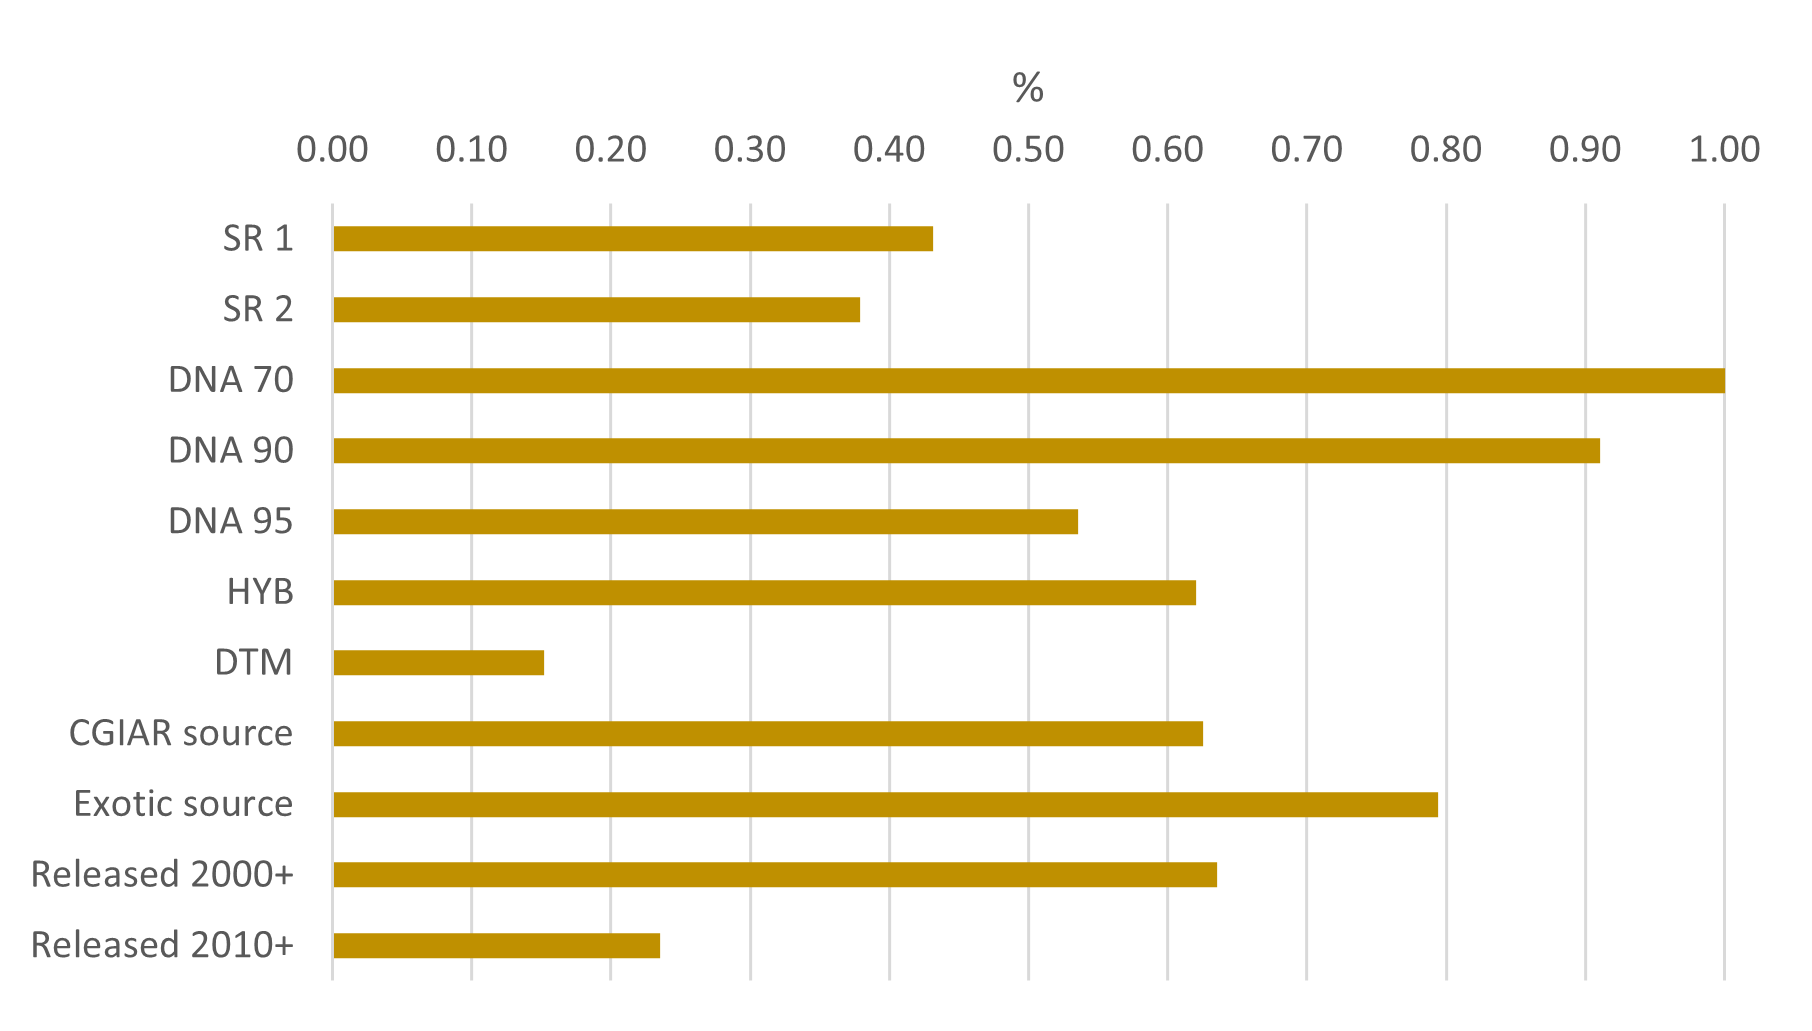
\includegraphics[width=.7\textwidth]{results/figures/adoption_r4.png}
    \begin{table}[H]
    \centering
        \begin{tabular}{p{0.7\textwidth}} 
            \begin{tablenotes}
                  \small
                  \item Note: Shares represent the proportion of adopters among maize farmers. Acronyms include: SR1 [=1 if New, 2nd gen or recycled, =0 if Traditional]; SR2  [=1 if New, =0 if 2nd gen, recycled or traditional]; DNA70 - Improved if purity $>=$70$\%$; DNA90 - Improved if purity $>=$90$\%$; DNA95 - Improved if purity $>=$95$\%$; HYB - Improved DNA, [=1 Hybrid, 0=Open pollinated]; DTM - Drought tolerant Maize [=1 DTM, 0=otherwise], CGIAR source [=1 if germplasm associated to a CGIAR-related thread], Exotic source [=1 if germplasm associated to an exotic source], Released 2000+ [=1 if DNA associated to a variety released on year 2000 or later], Released 2010+ [=1 if DNA associated to a variety released on year 2010 or later]. QPM is not included as there are too few households planting QPM seeds (n=6).
            \end{tablenotes}
        \end{tabular}
    \end{table}   
\end{figure}

We find regional variations in adoption levels. In the regions of Oromia, Amhara, Tigray, and SNNPR, around 39\% of households report adopting an improved varierty . In the regions of Amhara, Benishangul-Gumuz, Oromia, SNNPR, and Tigray, adoption rates of improved maize varieties were found for 27\% of households (\citealp{Jaleta2018-oj}). In Oromia, SNNPR, and Benishangul-Gumuz adoption of improved varieties per farmers’ self-reports was found for 84\% of maize growers in 2011, and 88\% of maize growers in 2013 (\citealp{Yirga17}).

Understanding the effects of improved seed adoption is not only challenging because there could be multiple ways of establishing what constitutes an improved seed, but also because such definitions may or may not overlap, or because farmers may also misclassify a variety as improved. Figure \ref{fig:missclassification} shows the correlation between the different definitions discussed above. For those seeds for which genetic material was obtained, the correlation with the self-reported seeds indicator is low, especially when using lower purity cutoff thresholds. 

\begin{figure}[htpb]
    \centering
    \caption{Correlation of different definitions of improved seeds, 4th round}\label{fig:missclassification}
    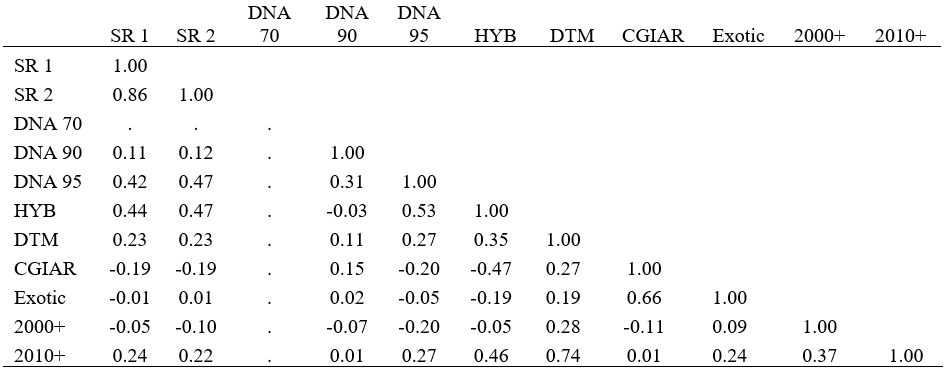
\includegraphics[width = 0.9\textwidth]{results/figures/missclassification.png}
    \vspace*{-2em}
    \begin{table}[H]
        \centering
        \begin{tabular}{p{1\textwidth}} 
            \begin{tablenotes}
                  \small
                  \item Note: Shares represent the proportion of adopters among maize farmers. Acronyms include: SR1 [=1 if New, 2nd gen or recycled, =0 if Traditional]; SR2  [=1 if New, =0 if 2nd gen, recycled or traditional]; DNA70 - Improved if purity $>=$70$\%$; DNA90 - Improved if purity $>=$90$\%$; DNA95 - Improved if purity $>=$95$\%$; HYB - Improved DNA, [=1 Hybrid, 0=Open pollinated]; DTM - Drought tolerant Maize [=1 DTM, 0=otherwise], CGIAR source [=1 if germplasm associated to a CGIAR-related thread], Exotic source [=1 if germplasm associated to an exotic source], Released 2000+ [=1 if DNA associated to a variety released on year 2000 or later], Released 2010+ [=1 if DNA associated to a variety released on year 2010 or later]. QPM is not included as there are too few households planting QPM seeds (n=6).
            \end{tablenotes}
        \end{tabular}
    \end{table}       
    
\end{figure}

\section{Estimation Strategy}\label{sec:strategy}

\subsection{Group Random Coefficient Model}

We use a Group Random Coefficients (GRC) approach to investigate the heterogeneous effects of adoption. The advantage of the GRC approach is that we do not rely on identification from a valid instrument, but on modeling the heterogeneity directly through a projection of adoption returns on their observed ``trajectory'' of adoption. This allows us to directly capture two effects: heterogeneous effects in the form of the so-called ``comparative advantage" of adoption, and, under the assumption of linearity in comparative advantage, a description of the overall economy's sorting of farmers based on their comparative advantage. The first is important because it is able to disentangle the effect of a general household's agricultural ability (which can be thought of as a fixed effect) and their adoption-specific potential. The second parameter can tell us whether the economy sorts farmers in a way that is commensurate with providing those that would benefit the most from adoption actually adopting, or whether there are barriers interfering with that. See \cite{Tjernstrom_Emilia_Dalia_Ghanem_Oscar_Barriga_Cabanillas_Travis_J_Lybbert_Jeffrey_D_Michler_and_Aleksandr_Michuda2020-bc} for more information on the assumptions involved for the GRC approach. 

% we contribute to the literature and methodology of \cite{Tjernstrom_Emilia_Dalia_Ghanem_Oscar_Barriga_Cabanillas_Travis_J_Lybbert_Jeffrey_D_Michler_and_Aleksandr_Michuda2020-bc} by providing reasonable ways to aggregate the results of the GRC model, which may seem difficult to interpret in its raw form. We use these aggregations to better understand the heterogeneous effects to adoption.

\afterpage{{\footnotesize\tabcolsep=1pt  % hold it local
    \centering
    \begin{table}
\centering
\caption{Trajectories of Households}
\label{tbl:trajectories}
\begin{tabular}{lrr}
\toprule
Trajectory &  Frequency &    Share \\
\midrule
       000 &       2124 & 0.611927 \\
       111 &        456 & 0.131374 \\
       011 &        228 & 0.065687 \\
       001 &        219 & 0.063094 \\
       010 &        153 & 0.044080 \\
       100 &        108 & 0.031115 \\
       110 &         96 & 0.027658 \\
       101 &         87 & 0.025065 \\
\bottomrule
\multicolumn{3}{l}{Note: Table shows frequency and shares of each trajectory in sample. 1 denotes adoption and 0 otherwise. The first digit is for whether the household adopted in wave 1, the second digit for wave and the third digit for wave 3}
\end{tabular}
\end{table}

    \vspace*{-4em}
    \begin{table}[H]
        \centering
        \begin{tabular}{p{0.7\textwidth}} 
            \begin{tablenotes}
                  \small
                  \item Note: Author's calculations using ESS. Maize farmers only. Table shows household adoption trajectories, their frequency and their share in the sample. 1 denotes adoption of improved maize seed, 0 otherwise. The first digit denotes adopting in wave 1, the second in wave 2, and the third in wave 3. 
            \end{tablenotes}
        \end{tabular}
    \end{table}  
    \newpage
}} 

Table \ref{tbl:trajectories} maps out the frequencies of the trajectories present in the data, sorted by frequency. Most households do not adopt at all (``never-adopters''), but the second most frequent trajectory are those that adopt in every wave (``always-adopters''). Let $\mathcal{H}$ be the set of these trajectories in the data and let $\mathcal{H}_S$ be the set of switcher trajectories, i.e. $\mathcal{H}_S = \mathcal{H}\backslash\{(0,0,0), (1,1,1)\}$

To generate results for adoption, we use the unrestricted model as outlined in \cite{Tjernstrom_Emilia_Dalia_Ghanem_Oscar_Barriga_Cabanillas_Travis_J_Lybbert_Jeffrey_D_Michler_and_Aleksandr_Michuda2020-bc}:

\begin{align}
y_{it}&=\sum_{\underline{h}\in\mathcal{H}\backslash (1,1,1)}\mu_{\underline{h}}+\sum_{\underline{h}\in\mathcal{H}_{S}}\Delta_{\underline{h}}h_{it}1\{h_{i}=\underline{h}\} + \kappa_{(1,1,1)}h_{it}1\{\underline{h}=(1,1,1)\}+ X_{it}\beta+\varepsilon_{it}.\label{eq:GRC}
\end{align}

where $y$ is log yields, $\mu_{\underline{h}}$ are binary variables for being in trajectory $\underline{h}$, $h$ is a binary variable for whether household $i$ adopted in wave $t$, and $X$ are a set of controls. $\kappa_{(1,1,1)}$ is the average yield with adoption of the always-adopters, where $\kappa_{(1,1,1)} = \mu_{(1,1,1)} + \Delta_{(1,1,1)}$. It is not possible to separately identify $\mu_{(1,1,1)}$ and $\Delta_{(1,1,1)}$ without adding more structure to the model in the form of the linearity in comparative advantage (LCA) restriction, which we explain how to test for below.

Our results use two definitions of yields: measured cropcuts of dry maize and self-reported maize yields. Each measure of yields has its benefits and drawbacks. Cropcuts, for instance, provide a true estimate of yields for a given parcel, but at the cost of a reduced sample size. Self-reports have larger sample sizes, but may suffer from measurement error \citep{gollin2021heterogeneity}. For controls we use the years of education of the household head, the age of the household head, the sex of the household head, whether there is a title for the land being cultivated, the parcel size in hectares, as well as the hours of household and hired labor. Commensurate with the literature, we also include interactions of these controls with improved seed adoption as added controls. Interactions with the improved seed variable are meant to further account for household specific variation that adopters may have. 

We estimate comparative advantage using the restricted model:

\begin{align}
y_{it}&=\sum_{\underline{h}\in\mathcal{H}\backslash (1,1,1)}\mu_{\underline{h}}+\Delta_{(0,0,1)}h_{it}+\phi(\mu_{(0,0,1)}-\mu_{(0,0,1)})h_{it}1\{h_{i}=(0,0,1)\}\nonumber\\
&~~~+\left(\mu_{(1,1,1)}+\phi\left(\mu_{(1,1,1)}-\mu_{(0,0,1)}\right)\right)h_{it}1\{h_{i}=(1,1,1)\} + X_{it}\beta +\varepsilon_{it},\label{eq:GRC_Suri}
\end{align}

where $\phi$ is the parameter which describes sorting in the economy and $\Delta_{0,0,1}$ are the returns to adoption for trajectory $(0,0,1)$. If $\phi$ is positive, then higher yields are associated with higher comparative advantage, denoting that those that adopt also tend to have the highest returns to adoption. If it is negative, however, it implies farmers who do better on average see a worse yield performance while using improved seeds. A results that can reflect  barriers, such as a lack of fertilizer access, and bad roads that restrict the ability to buy hybrid seed. We estimate $\phi$ in two ways: through the restricted model just mentioned and by a weak-identification grid procedure, which allows for calculating the confidence interval for $\phi$ for multiple sets of trajectories. The advantage of the weak-identification robust procedure is that we can test for whether the data satisfies the conditions necessary for an interpretable $\phi$ parameter, before estimating the restricted model. If there are trajectories which yield a $\phi$ with a non-infinite confidence interval, then the LCA is at least partially satisfied.

Equation \ref{eq:GRC_Suri} can be estimated by way of General Method of Moments. Parameters for returns to adoption and comparative advantage can be post-estimated by the delta method, where the expression for returns of each trajectory can be derived from:

$$
\Delta_{\underline{h}}=\phi\left(\mu_{\underline{h}}-\mu_{(0,0,1)}\right) + \Delta_{(0,0,1)}
$$

for trajectory $\underline{h} \neq (0,0,1)$.\footnote{Since we use $(0,0,1)$ as our base, we already have returns available for that trajectory, namely $\Delta_{(0,0,1)}$} Comparative advantage can be derived from:

$$
\theta_{\underline{h}} = \mu_{\underline{h}} - E(\mu_{\underline{h}})
$$

where $E(\mu_{\underline{h}}) = \sum_{\mathcal{H}} \pi_h \cdot \mu_h$ for $\pi_h$ being the frequency weight for trajectory $h$. The comparative advantage of each trajectory tells us how much a household with a given trajectory benefits from adoption. $\theta <0 $ denotes that adoption-specific potential is negative and that a household loses by adopting.

% Once we generate $\theta$ and $\Delta$ for each trajectory, we can examine heterogeneous effects to adoption. Conditional on the LCA being satisfied, that means that there will be eight comparative advantages available for comparison, which is rich in its information, but difficult to interpret. As a result, we will aggregate $\theta$ in two ways to improve interpretability: (1) by which wave the household adopted, and (2) the number of times adoption took place. We do this by taking a simple average, grouped by each of these factors. The first aggregation will tell us whether there are any wave-specific differences in comparative advantage. The second aggregation will tell us whether adopting more times corresponds to higher comparative advantage and associated returns. In both cases, these aggregations reflect the economic landscape that drive returns to adoption.

% To compare the results when using a dichotomous adoption decision with an intensity of adoption variable, we run a similar regression to the above to calculate the comparative advantage of adopting a certain number of times. We estimate an equation similar to Eq. \ref{eq:GRC_Suri}, but use the number of times that a household adopted an improved maize variety (here, $NAdopt$), not its trajectory.

% \begin{align}
% y_{it}&=\sum_{\underline{na}\in\mathcal{NA}\backslash 3}\nu_{\underline{h}}+\Delta_{(0,0,1)}h_{it}+\phi(\nu_{(0,0,1)}-\nu_{(0,0,1)})_{it}1\{NAdopt_{i}=1\}\nonumber\\
% &~~~+\left(\nu_{(1,1,1)}+\phi\left(\nu_{(1,1,1)}-\nu_{(0,0,1)}\right)\right)h_{it}1\{NAdopt_{i}=3\} + X_{it}\beta +\varepsilon_{it},\label{eq:GRC_NAdopt}
% \end{align}

% Here instead of a set of trajectories, we have a set of the number of times adopted $\mathcal{NA}$. $\nu$ denotes the average yield from adoption $na$ times. We use adopting once as the base.

\subsection{Endogenous Switching Regression}

The GRC approach uses the variation in the adoption trajectories of each household in the ESS 1-3 panel as a source of information that allows for an unbiased estimation. However, because it only includes self-reported use of improved seed, estimates may suffer from missclassification bias. We hence use the  DNA-fingerprinting available in ESS4 to explore possible missclassification dynamics that may better inform the results from ESS 1-3. We propose an endogenous switching regression model to account for unobserved heterogeneity in adoption decisions. This method imposes restrictive assumptions regarding the distribution of the errors for the selection (into adoption) and output equations. At the same time, the exclusion restriction needs to be satisfied in order to reduce the bias of the estimation. 

The endogenous switching regression holds certain advantages over other methodologies used for identifying unbiased estimates with cross-sectional observational data such as propensity score matching or other instrumental variable approaches (\citealp{Shiferaw2014-op}) and has been used to study similar questions in the past (\citealp{falco2011does}; \citealp{kabunga2012yield}). \par
This approach models the effect of improved seed adoption on yields in two stages. First, the decision to adopt an improved seed is determined by a series of observed and unobserved variables. Equation \ref{eq:switch_latent} shows the definition for a latent variable $A^*$ that reflects the benefit from adopting an improved seed relative to planting a traditional one. As shown in the equation, household $i$ will decide to adopt ($A_i$=1) if these perceived benefits of adoption are positive.

\begin{align}
A_i^*=\bm{Z}_i\alpha+\varepsilon_i \; \text{with} \, A_i    \begin{cases}
      1, & \text{if}\ A_i^*>0 \\
      0, & \text{otherwise}
    \end{cases} \label{eq:switch_latent}
\end{align}

Vector $\bm{Z}$ includes variables that determine if a particular household may benefit from the adoption of improved seeds, such as farmers' demographic characteristics (education, age, female headed households) and land tenure status of their plots. In the estimations presented in the next sections, we consider different definitions of improved seeds, and include not only self-reported seed classification but also the results of DNA fingerprinting.  \par
The second stage presents the outcome functions conditional on adoption, where farmers choose between adopting an improved seed (regime 1) or using a traditional seed (regime 2):
\begin{align}
    \text{Regime 1}: \; y_{1i}=\bm{X}_{1i}\beta_1+ \epsilon_{1i} \; if \; A_i=1 \label{eq:switch_reg1}\\
     \text{Regime 2}: \; y_{2i}=\bm{X}_{2i}\beta_1+ \epsilon_{2i} \; if \; A_i=0 \label{eq:switch_reg2} 
\end{align}
$y_{1i}$ and $y_{2i}$ are yields under regime 1 or regime 2 for household $i$, and $\bm{X}$ is a vector of variables that affect yields including parcel size, household and hired labor, costs of fertilizers and other inputs, whether the household has access to irrigation or farm mechanization, among others.  \par
The model assumes that the error terms of Equations \ref{eq:switch_latent}, \ref{eq:switch_reg1}, \ref{eq:switch_reg2} have a trivariate normal distribution with mean equal to 0 and a covariance matrix with diagonal terms equal to $\sigma_{\varepsilon}^2$, $\sigma_1^2$ $\sigma_2^2$, and non-zero covariances between $\varepsilon$ and $\epsilon_1$ ($\sigma_{1\varepsilon}$) and between $\varepsilon$ and $\epsilon_2$ ($\sigma_{2\varepsilon}$), and not defined between $\epsilon_1$ and $\epsilon_2$ since both regimes are not observed simultaneously for any given $i$. This error structure is derived from the expected value $\epsilon_1$ ($\epsilon_2$) conditional on adoption  (non-adoption) respectively to be non-zero, reflecting the endogeneity in the adoption decision. These conditional expectations are equal to:
\begin{align*}
    E(\epsilon_{1i}|A_i=1)=&\sigma_{1\varepsilon}\frac{\phi(\bm{Z}_i\alpha)}{\Phi(\bm{Z}_i\alpha)}=\sigma_{1\varepsilon}\lambda_{1i} \\
    E(\epsilon_{2i}|A_i=0)=&-\sigma_{2\varepsilon}\frac{\phi(\bm{Z}_i\alpha)}{(1-\Phi(\bm{Z}_i\alpha))}=\sigma_{2\varepsilon}\lambda_{2i}
\end{align*}
%
where $\phi(\cdot)$ and $\Phi(\cdot)$ are the standard normal probability density and cumulative density functions, $\lambda_{1i}=\sigma_{1\varepsilon}\frac{\phi(\bm{Z}_i\alpha)}{\Phi(\bm{Z}_i\alpha)}$ and $\lambda_{2i}=-\sigma_{2\varepsilon}\frac{\phi(\bm{Z}_i\alpha)}{(1-\Phi(\bm{Z}_i\alpha))}$. \par

We estimate this model simultaneously using maximum likelihood estimation following \cite{lokshin2004maximum}, which accounts for the endogeneity in the yield equation.  Statistically significant estimates for the covariances $\sigma_{1\varepsilon}$ and $\sigma_{2\varepsilon}$ indicate the presence of endogeneity in the adoption and yield equations. 


A key advantage of this approach is that it allows us to compare the expected yields for adopters under the two regimes, the observed (adoption) and the counterfactual (non-adoption). This effect is the Average Treatment Effect on the Treated (ATT). Analogously, it is also possible to calculate the Average Treatment Effect on the Untreated (ATU) by comparing expected yields under the two regimes for non-adopters: the counterfactual (adoption) and the observed (non-adoption). The following equations present the expected yield equations for adopters and non-adopters under both regimes:

\begin{subequations}
\begin{align}
    E(y_{1i}|A_i=1)=\bm{X}_1i\beta_1+\sigma_{1\varepsilon} \lambda_{1i} \label{eq:att_1} \\
    E(y_{2i}|A_i=1)=\bm{X}_1i\beta_2+\sigma_{2\varepsilon} \lambda_{1i} \label{eq:att_0} \\
    E(y_{2i}|A_i=0)=\bm{X}_2i\beta_2+\sigma_{2\varepsilon} \lambda_{2i} \label{eq:atu_0} \\
    E(y_{1i}|A_i=0)=\bm{X}_2i\beta_1+\sigma_{1\varepsilon} \lambda_{2i} \label{eq:atu_1}    
\end{align}
\end{subequations}

The ATT is equal to the difference between Equation \ref{eq:att_1} and Equation \ref{eq:att_0}. The ATU is the difference between Equation \ref{eq:atu_0} and Equation \ref{eq:atu_1}. Note that the observed expectations are those linked to Equations \ref{eq:att_1} and \ref{eq:atu_0} for adopters and non-adopters, while the counterfactual expectations are those presented in Equations \ref{eq:att_0} and \ref{eq:atu_1} respectively. We report these results with bootstrapped standard errors in order to measure the yield benefit of adoption for adopters and non-adopters. 

\subsection{Misclassification-Robust GRC}

As a last step, we introduce a misclassification-robust approach to the GRC method, which allows us to take misclassification into account when calculating comparative advantage. Using the DNA identification from ESS4 we are able to verify how often an improved seed is actually used when a farmer self-reports adopting improved seed. The methodology in this section builds on work that was done in \cite{michuda2021three}, which used confusion matrices from machine learning algorithms as a way to estimate a causal effect that was robust to misclassification. Misclassification introduces non-classical measurement error that may attenuate estimates and bias them towards 0 in the binary case. In the multi-regime case, misclassification will tend to make estimates too close to one another, leading to smaller or even wrong-signed estimates.

Let $p_{ij}$ be the $i,j$th cell of a two by two misclassification matrix. Suppose that we construct the probability of being in a true trajectory $h = (i,j,k)$, intersected with being in a reported trajectory $\hat{h} = (\hat{i},\hat{j}, \hat{k})$ as:

\begin{equation}
\label{eq:misclass}
P(h = (i,j,k) , \hat{h} = (\hat{i},\hat{j}, \hat{k})) = p_{i, \hat{i}}\cdot p_{j, \hat{j}}\cdot p_{k, \hat{k}}
\end{equation}

We can use Eq. \ref{eq:misclass} to construct the joint distribution, $f(h, \hat{h})$ for each trajectory in the sample. 

Once we construct these probabilities, we estimate a Nonlinear-Maximum Likelihood function that is robust to misclassification. Essentially, this involves using the likelihood function obtained from the confusion matrices and apply it on the estimation of Eq. \ref{eq:GRC} as a conditional distribution of agricultural yield. The likelihood for one observation in this case would then be:

\begin{equation}
\label{eq:mr-grc}
l(\mu, \kappa, \Delta, \beta, \sigma|y_{t}, \hat{h}) = \sum_{\underbar{$h$}\in\mathcal{H}} \left[ f_{Y_{t}| \mathcal{H}}(y|h=\underbar{$h$})\cdot  \sum_{\bar{h} \in \mathcal{H}} 1\{\hat{h}=\bar{h}\} p_{\underbar{$h$}, \bar{h}} \right]
\end{equation}

\noindent where $1$ is the indicator function and $f$ is the probability distribution function conditional on true adoption assignment. We assume that this distribution is normal and can be written with a mean of $y_t - \sum_{\underline{h}\in\mathcal{H}\backslash (1,1,1)}\mu_{\underline{h}}-\sum_{\underline{h}\in\mathcal{H}_{S}}\Delta_{\underline{h}}h_{it}1\{h_{i}=\underline{h}\} - \kappa_{(1,1,1)}h_{it}1\{\underline{h}=(1,1,1)\}- X_{it}\beta$ and some nuisance variance parameter $\sigma$, which is estimated. Put more succinctly, we use Eq. \ref{eq:GRC} in the normal distribution. We will call this estimator, Misclassification-Robust GRC.\footnote{For more information on the derivation of the original estimator, as well as a link to a python package of its implementation, see \cite{michuda2021three}.}


\section{Results}\label{sec:results}

\subsection{Group Random Coefficients}



%  self-reported yields are systematically higher than cropcut yields, pointing to the fact that there may be some measurement error at play. 

Figure \ref{fig:theta_delta_raw} shows a plot of the comparative advantages and returns for the cropcuts model with controls (full results for both self-report and cropcuts are shown in the Appendix). These results highlight two interesting puzzles: it would seem that for many trajectories, comparative advantage is either very close to 0, implying that there is no difference between farmers that adopt and not adopt. For trajectory $(0,1,1)$, comparative advantage is exceedingly negative. This is peculiar, as this would imply that farmers that adopted in both waves 2 and 3 would actually be better off not adopting, even though their returns are positive (as shown in the bottom figure). Another peculiarity in this figure is that it would seem that if we compare trajectories that only differ by one wave's adoption, comparative advantage and returns seem to fall. For example, the transition from $(0,1,0)$ to $(0,1,1)$ leads to a large fall in comparative advantage. The same can be seen less starkly for the move from $(1,0,0)$ to $(1,0,1)$ and $(1,1,0)$ to $(1,1,1)$. But despite this loss in comparative advantage, returns seem to increase. This seems to imply that adopting more often leads to higher comparative advantage, but slightly higher returns. 

\begin{figure}
    \centering
    \caption{Comparative Advantage and Returns by Trajectory (Dry Cropcuts)}
    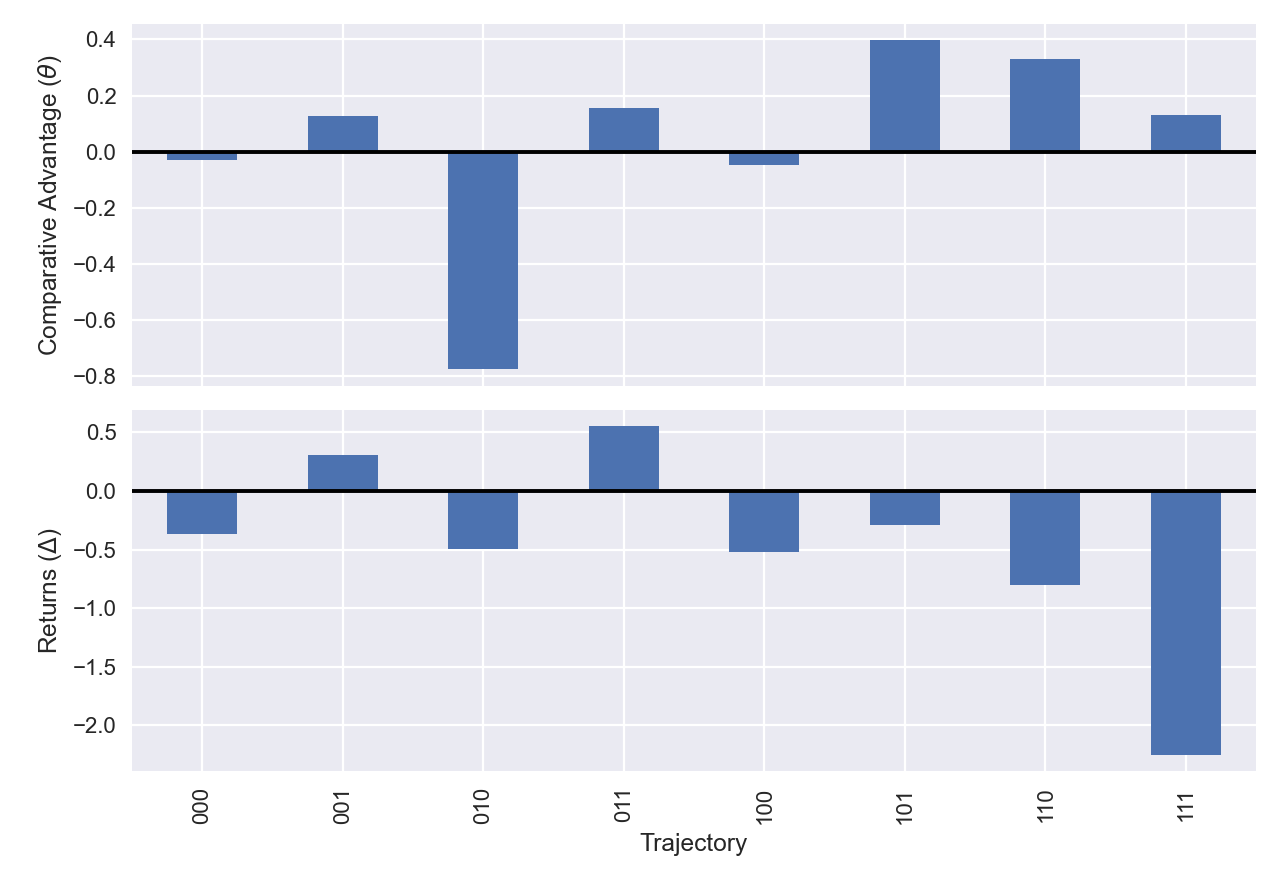
\includegraphics[scale=0.7]{results/figures/theta.png}\label{fig:theta_delta_raw}
        \vspace*{-2em}
    \begin{table}[H]
        \centering
        \begin{tabular}{p{0.8\textwidth}} 
            \begin{tablenotes}
                  \small
                  \item Note: Author's calculations using ESS. The figures shows the comparative advantage and the returns to adoption for each adoption trajectory. Log(Dry cropcuts) used as outcome. Top figure denotes comparative advantage for each trajectory. Bottom figure denotes returns to adoption for each trajectory.
            \end{tablenotes}
        \end{tabular}
    \end{table}
\end{figure}

% We then estimate the GRC equation replacing the binary adoption variable by the number of times a farmer adopted an improved variety. Figure \ref{fig:n_adopt} shows the results and the calculation of the comparative advantage. As expected, adopting zero times leads to negative comparative advantage, but with positive returns to adoption, implying that there is value to adopting to those that have never adopted hybrid maize seed. Adopting once leads to both positive comparative advantage, and positive returns to adoption. However, adopting twice actually leads to negative comparative advantage, and less positive returns. Adopting all three times leads to positive comparative advantage, but negative returns.

% \begin{figure}
%     \centering
%     \caption{Aggregation Results: Comparative Advantage and Returns by the Number of Times Adopted (Dry Cropcuts)}
%     \label{fig:n_adopt}
%     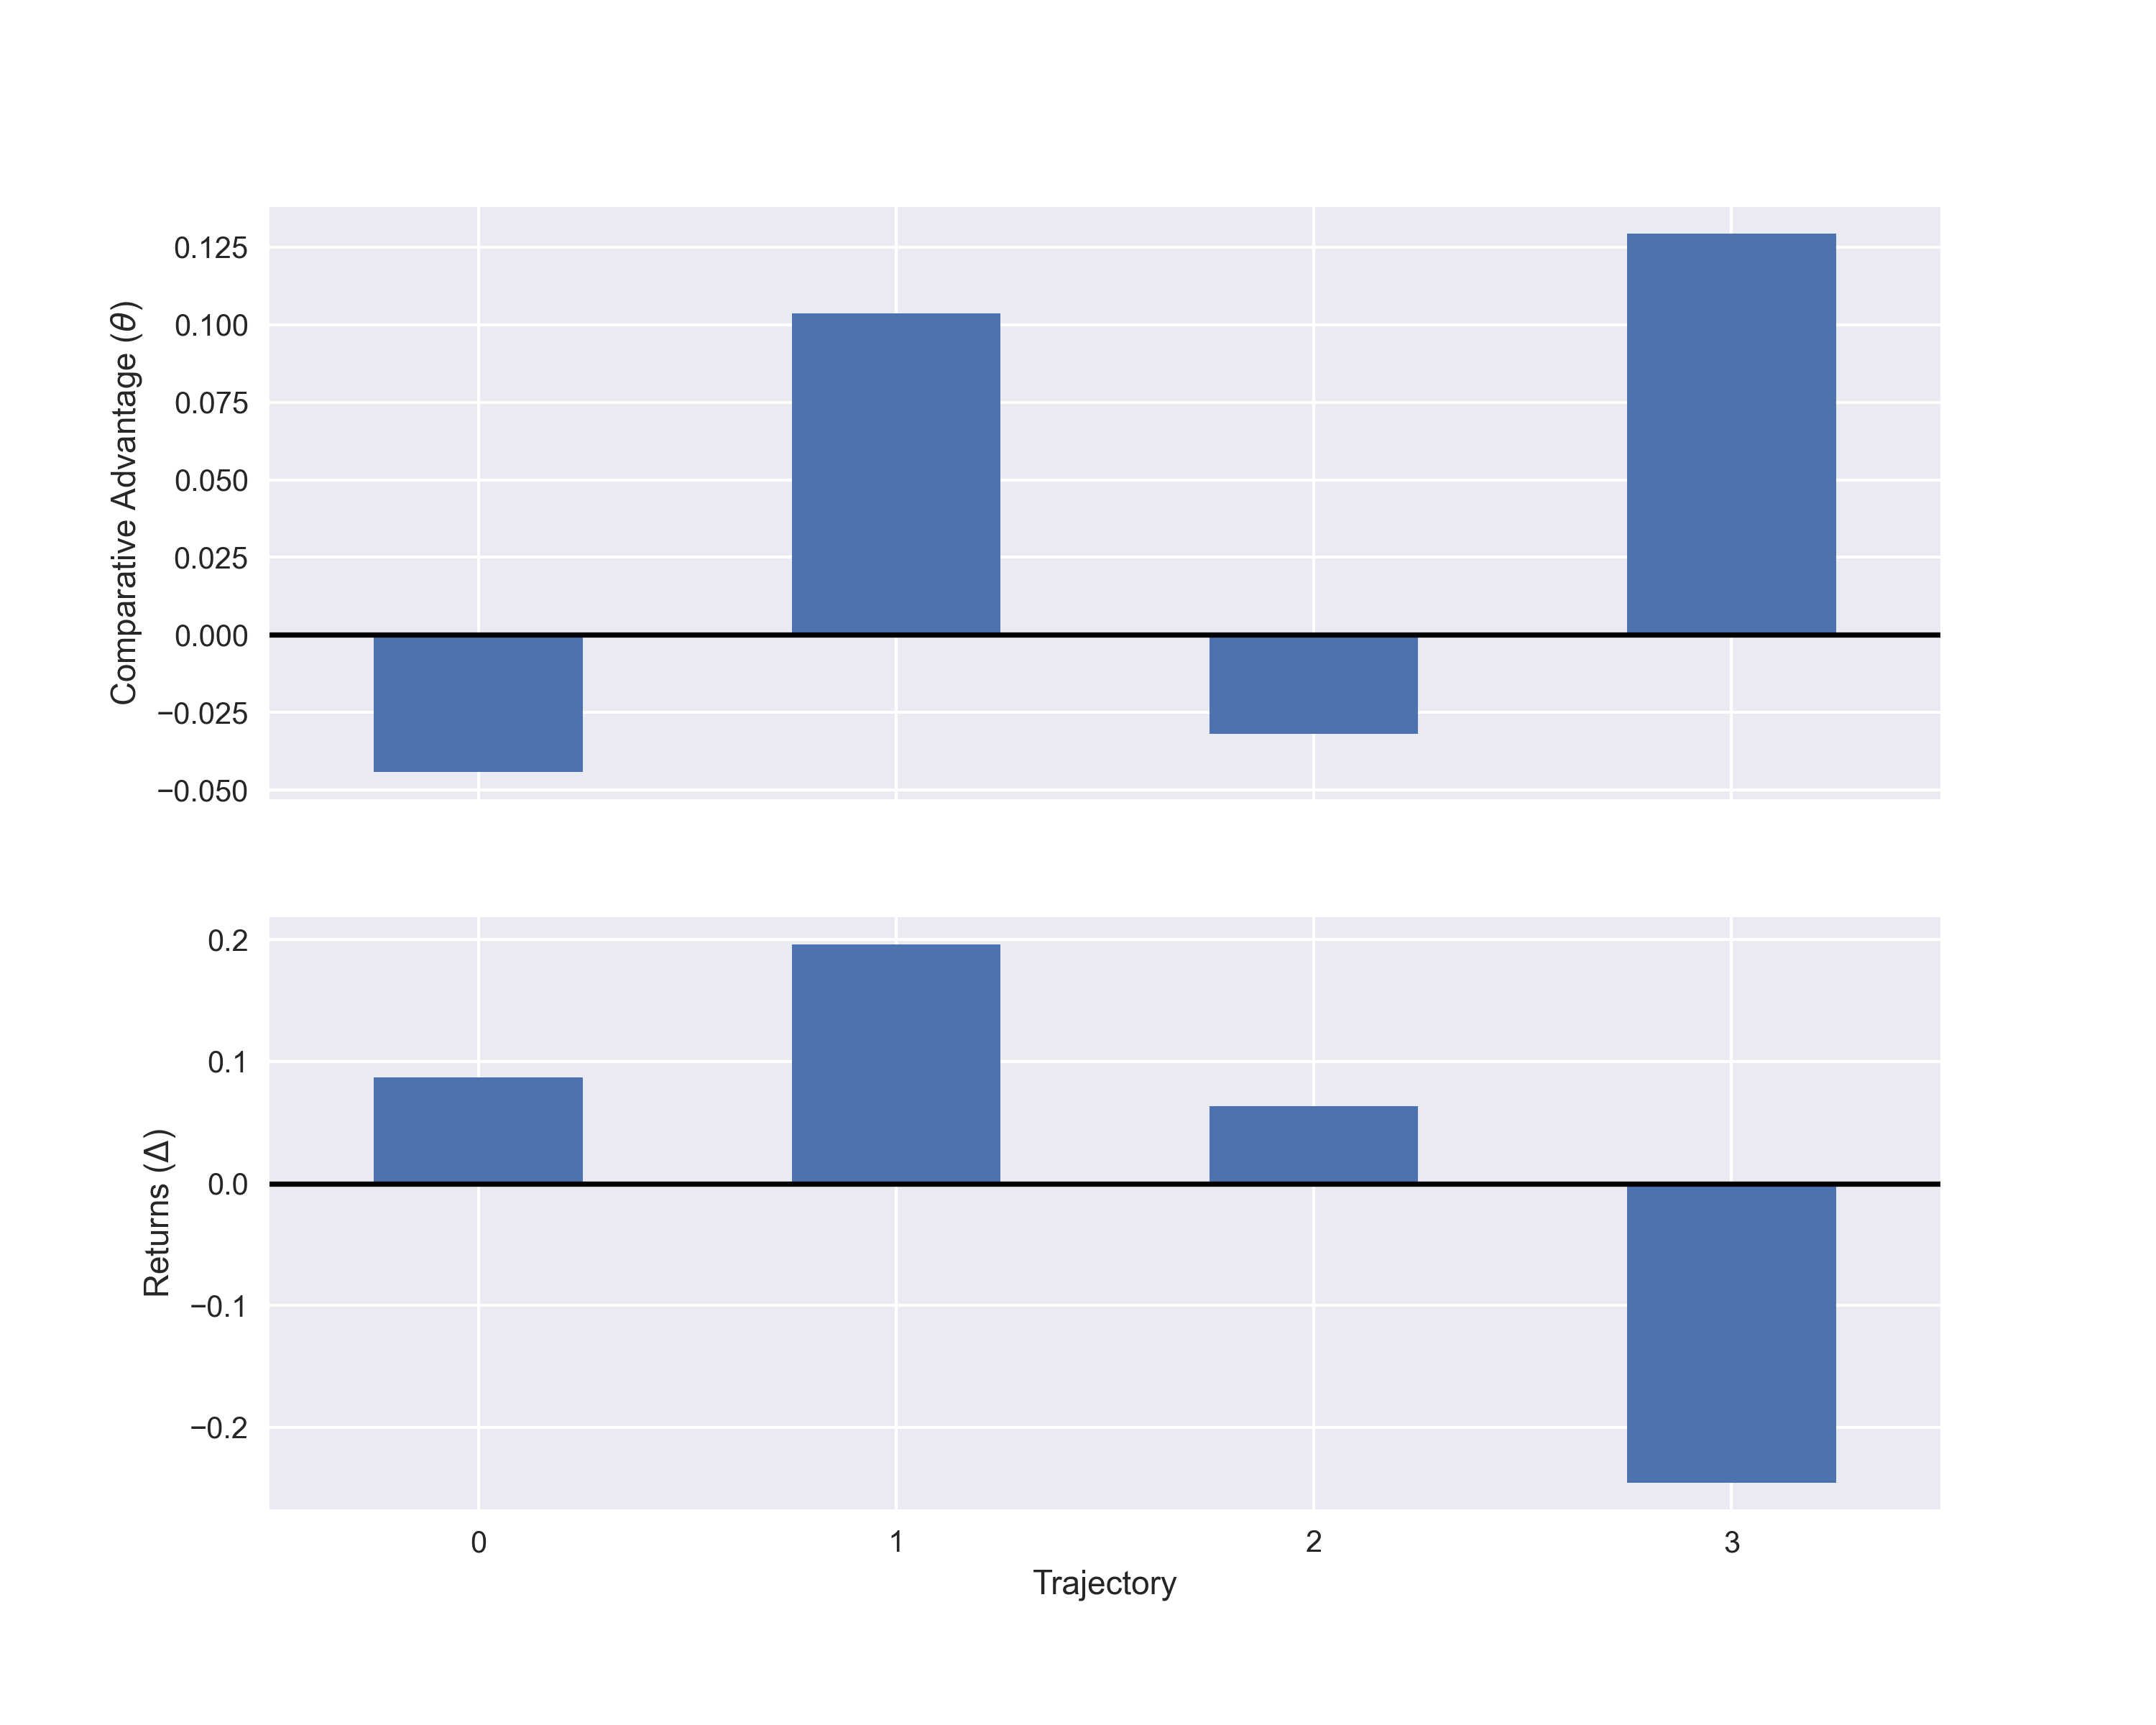
\includegraphics[scale=0.75]{results/figures/num_adoption.png}
%     \vspace*{-2em}
%     \begin{table}[H]
%         \centering
%         \begin{tabular}{p{0.75\textwidth}} 
%             \begin{tablenotes}
%                   \small
%                   \item Note: Author's calculations using ESS. The figures shows the aggregate impact from Table \ref{tbl:unres} using the number of time a person adopted as the basis for the aggregation.
%             \end{tablenotes}
%         \end{tabular}
%     \end{table}
% \end{figure}



\subsection{Endogenous Switching Regression}

To complement the results of the GRC model, we present the Endogenous Switching Regression results. We first examine a self-reported definition of an improved variety to validate the results from the GRC model. As before, we consider a looser definition of improved seeds, which includes new seeds but also second-generation and recycled (SR1), and a more strict definition, which includes only new varieties (SR2). Table \ref{tab:switch1} shows the results of the Switching regression using both definitions, and using self-reported and cropcut yields. We see that regardless of the definition of improved seed, yield measurement and controls included, the results consistently show that the ATT is negative and the ATU is positive, meaning that farmers that adopted a self-reported improved seed would've been better off not adopting. Farmers that did not adopt improved seeds would have been better off adopting. This is in line with the GRC results as it seems to imply that households are not making profit-maximizing decisions; their adoption decisions seem to be leading to a reduction in welfare, whether they are adopting or not adopting.

\begin{table}[H]
\centering
\hspace*{-1.2cm}
\begin{threeparttable}
\caption{Effects on yields (log) from adopting improved maize varieties (self-reported)}
\label{tab:switch1}
\begin{tabular}{l cccccc}
\hline
\hline
            &Adopters yields&Non-adopters yields&         ATE&          SE&     p-value\\
\hline
\textit{SR1, SR yields}&            &            &            &            &            \\
ATT         &        7.30&        9.07&       -1.76&       0.011&      0.0000\\
%
%
%
ATU         &        9.06&        6.87&        2.19&       0.024&      0.0000\\
%
%
%
\textit{SR1, cropcut yields}&            &            &            &            &            \\
ATT         &        7.57&        7.86&       -0.30&       0.017&      0.0000\\
%
%
%
ATU         &        8.89&        7.11&        1.78&       0.039&      0.0000\\
%
%
%
\textit{SR1, SR yields, full set of controls}&            &            &            &            &            \\
ATT         &        7.28&        7.82&       -0.54&       0.019&      0.0000\\
%
%
%
ATU         &        9.65&        6.85&        2.80&       0.100&      0.0000\\
%
%
%
\textit{SR1, cropcut yields, full set of controls}&            &            &            &            &            \\
ATT         &        7.56&        7.61&      -0.049&       0.019&      0.0087\\
%
%
%
ATU         &        9.24&        7.11&        2.13&       0.085&      0.0000\\
%
%
%
\textit{SR2, SR yields}&            &            &            &            &            \\
ATT         &        7.30&        7.85&       -0.55&       0.020&      0.0000\\
%
%
%
ATU         &        9.63&        6.88&        2.75&       0.101&      0.0000\\
%
%
%
\textit{SR2, cropcut yields}&            &            &            &            &            \\
ATT         &        7.61&        7.62&      -0.013&       0.019&        0.47\\
%
%
%
ATU         &        9.35&        7.14&        2.21&       0.091&    1.6e-130\\
\hline
\hline
\end{tabular}
\begin{tablenotes}
\footnotesize
\item{Note: Full set of controls include: parcel size (in HA), household labor, hired labor, fertilizer costs, other input costs irrigation (dummy), mechanization (dummy), organic fertilizer (dummy). Instruments for the adoption equation include: years of education of hh head, age of hh head, female head, land title, asset index, seed costs. Results for SR2 include full set of controls. SR1=1 if New, 2nd gen or recycled,=0 if Traditional; SR2=1 if New, =0 2nd gen, recycled or traditional}
\end{tablenotes}
\end{threeparttable}
\end{table}


To better understand the above puzzling results, we explore similar yield estimations using the different definitions of improved seed from DNA fingerprinting. The DNA fingerprinting data allows us to be confident in whether a seed that was used, was in fact improved. We run similar switching regressions using different thresholds of DNA purity (70, 90 and 95\% purity), hybrid vs. open-pollinated varieties, and drought-tolerant maize (DTMZ). Table \ref{tab:switch2} shows the results. 

The results show that the initial switching regression results and the GRC results could be driven by seed definition. All the plots sampled for DNA fingerprinting showed a purity percent of 70\% or higher, which means that even farmers that report using traditional seed only, could be in fact still using a 70\% mix with hybrid seed. This implies that we need a counter-factual to compare these purity thresholds with non-adopters. We consider non-adopters those who self-reported using a traditional variety. Given the universality of improved varieties with a 70\% threshold or higher and given the high rates of misclassification, the control group for a 70\% threshold is likely to be contaminated with a high share of false positives. But the results are biased downwards and the control group for higher shares of purity will be less contaminated. 

Table \ref{tab:switch2} shows that the estimations for purity thresholds of 70 and 90\% show similar patterns as before: non-adopters would've been better off adopting and adopters would've been better off not adopting. However, when we use a 95\% purity definition, the ATT becomes positive and the ATU is still positive but significantly reduced (and even negative when self-reported yields are used). Farmers that adopted a variety with a 95\% purity or greater had significantly greater yields than if they had not adopted. 

We get similar results for DTMZ. Farmers that adopt DTMZ (as tracked by the DNA germplasm) did obtain greater yields than if they had not adopted. Again, this result may be biased downwards because of possible false-positives among the control group. The results for the comparison between hybrid and open-pollinated varieties are not significant (when using self-reported yields).

\begin{table}[H]
\centering
\hspace*{-1.2cm}
\begin{threeparttable}
\caption{Effects on yields (log) from adopting improved maize varieties (DNA fingerprinting)}
\label{tab:switch2}
\begin{tabular}{l cccccc}
\hline
\hline
            &Adopters yields&Non-adopters yields&         ATE&          SE&     p-value\\
\hline
\textit{DNA 70, SR yields}&            &            &            &            &            \\
ATT         &        7.17&        7.31&       -0.14&       0.026&      0.0000\\
%
%
%
ATU         &        8.76&        6.76&        2.00&       0.036&      0.0000\\
%
%
%
\textit{DNA 70, cropcut yields}&            &            &            &            &            \\
ATT         &        7.28&        8.48&       -1.21&       0.041&      0.0000\\
%
%
%
ATU         &        8.55&        7.27&        1.28&       0.042&      0.0000\\
%
%
%
\textit{DNA 90, SR yields}&            &            &            &            &            \\
ATT         &        7.18&        9.07&       -1.90&       0.023&      0.0000\\
%
%
%
ATU         &        7.01&        6.80&        0.21&       0.022&      0.0000\\
%
%
%
\textit{DNA 90, cropcut yields}&            &            &            &            &            \\
ATT         &        7.30&        8.72&       -1.43&       0.028&      0.0000\\
%
%
%
ATU         &        9.32&        7.24&        2.09&       0.034&      0.0000\\
%
%
%
\textit{DNA 95, SR yields}&            &            &            &            &            \\
ATT         &        7.30&        7.08&        0.22&       0.036&      0.0000\\
%
%
%
ATU         &        6.87&        6.86&       0.018&       0.029&      0.5496\\
%
%
%
\textit{DNA 95, cropcut yields}&            &            &            &            &            \\
ATT         &        7.52&        7.39&        0.13&       0.018&      0.0000\\
%
%
%
ATU         &        7.38&        7.12&        0.26&       0.024&      0.0000\\
%
%
%
\textit{HYB, SR yields}&            &            &            &            &            \\
ATT         &        7.28&        7.25&       0.030&       0.028&      0.2892\\
%
%
%
ATU         &        7.06&        6.85&        0.21&       0.028&      0.0000\\
%
%
%
\textit{HYB, cropcut yields}&            &            &            &            &            \\
ATT         &        7.51&        7.55&      -0.038&       0.017&      0.0289\\
%
%
%
ATU         &        7.58&        7.03&        0.55&       0.021&      0.0000\\
%
%
%
\textit{DTMZ, SR yields}&            &            &            &            &            \\
ATT         &        7.42&        6.53&        0.89&       0.074&      0.0000\\
%
%
%
ATU         &        7.11&        7.02&       0.089&       0.022&      0.0001\\
%
%
%
\textit{DTMZ, cropcut yields}&            &            &            &            &            \\
ATT         &        7.56&        6.76&        0.81&       0.058&     3.5e-44\\
%
%
%
ATU         &        8.04&        7.27&        0.77&       0.028&    9.4e-167\\
\hline
\hline
\end{tabular}
\begin{tablenotes}
\footnotesize
\item{Note: Full set of controls include: parcel size (in HA), household labor, hired labor, fertilizer costs, other input costs irrigation (dummy), mechanization (dummy), organic fertilizer (dummy). Instruments for the adoption equation include: years of education of hh head, age of hh head, female head, land title, asset index, seed costs. All results include full set of controls. DNA 70, 90 and 95 refer to improved varieties defined by DNA finerprinting with purity levels of 70, 90 and 95\%, respectively. HYB equals 1 for a hybrid variety, 0 for an open-pollinated variety. DTMZ equals 1 for a Drought-tolerant maize variety}
\end{tablenotes}
\end{threeparttable}
\end{table}


To further disaggregate the results, we explore the source of the improved varieties (CGIAR or exotic) and the year of the seed release. These results are shown in Table \ref{tab:switch3}. We find positive effects for adopters of CGIAR-sourced varieties when using self-reported yields. The results seem to be contradictory when using cropcut yields, but we should consider these are different samples, as cropcuts were obtained in a subsample of plots. Exotic-sourced varieties also show positive yield effects for adopters; and a negative ATU, meaning non-adopters are also better off not adopting. Newly released-seed varieties do consistently show positive ATT, when using both self-reported and cropcut yields. 

\begin{table}[H]
\centering
\resizebox{0.8\textwidth}{!}{
\hspace*{-1.2cm}
\begin{threeparttable}
\caption{Effects on yields (log) from adopting improved maize varieties (DNA fingerprinting)}
\label{tab:switch3}
\begin{tabular}{l cccccc}
\hline
\hline
            &Adopters yields&Non-adopters yields&         ATE&          SE&     p-value\\
\hline
\textit{CGIAR source, SR yields}&            &            &            &            &            \\
ATT         &        7.13&        6.71&        0.43&       0.033&      0.0000\\
%
%
%
ATU         &        9.19&        6.89&        2.31&       0.018&      0.0000\\
%
%
%
\textit{CGIAR source, cropcut yields}&            &            &            &            &            \\
ATT         &        7.23&        8.98&       -1.75&       0.040&      0.0000\\
%
%
%
ATU         &        7.51&        7.40&        0.11&       0.015&      0.0000\\
%
%
%
\textit{Exotic source, SR yields}&            &            &            &            &            \\
ATT         &        7.13&        6.65&        0.48&       0.022&      0.0000\\
%
%
%
ATU         &        6.83&        6.89&      -0.060&       0.021&      0.0047\\
%
%
%
\textit{Exotic source, cropcut yields}&            &            &            &            &            \\
ATT         &        7.28&        7.18&       0.098&       0.032&      0.0023\\
%
%
%
ATU         &        6.73&        7.33&       -0.60&       0.021&      0.0000\\
%
%
%
\textit{Year 2000+, SR yields}&            &            &            &            &            \\
ATT         &        7.26&        5.55&        1.71&       0.046&      0.0000\\
%
%
%
ATU         &        8.87&        6.93&        1.94&       0.041&      0.0000\\
%
%
%
\textit{Year 2000+, cropcut yields}&            &            &            &            &            \\
ATT         &        7.55&        7.27&        0.28&       0.024&      0.0000\\
%
%
%
ATU         &        8.52&        7.25&        1.27&       0.027&      0.0000\\
%
%
%
\textit{Year 2010+, SR yields}&            &            &            &            &            \\
ATT         &        7.44&        6.92&        0.53&       0.039&      0.0000\\
%
%
%
ATU         &        8.98&        6.91&        2.07&       0.056&      0.0000\\
%
%
%
\textit{Year 2010+, cropcut yields}&            &            &            &            &            \\
ATT         &        7.57&        6.97&        0.60&       0.035&     8.6e-65\\
%
%
%
ATU         &        8.72&        7.25&        1.47&       0.019&           0\\
\hline
\hline
\end{tabular}
\begin{tablenotes}[flushleft]
\footnotesize
\item{Note: Full set of controls include: parcel size (in HA), household labor, hired labor, fertilizer costs, other input costs irrigation (dummy), mechanization (dummy), organic fertilizer (dummy). Instruments for the adoption equation include: years of education of hh head, age of hh head, female head, land title, asset index, seed costs. All results include full set of controls. }
\end{tablenotes}
\end{threeparttable}
}
\end{table}


\subsection{Misclassification-Robust GRC}

The previous results highlight the fact that the definition of improved seed matters. Even when households think they are not adopting hybrid maize seed, there is such a large amount of hybrid seed that has been introduced over the years in Ethiopia that farmers may be misclassifying their seed and taking part in sub-optimal growing strategies as a result. For instance, if a farmer thinks they are growing traditional seed, but they are actually growing hybrid seed, returns to adoption may be low, since hybrid seeds often require more fertilizer and inputs to work optimally.\footnote{If they are cultivated like traditional seeds, then their performance may end up being worse.}

We construct a confusion matrix based on the DNA fingerprinting data in the fourth wave and apply it to the previous three waves. Table \ref{tab:misclassification} shows a table of different hybrid seed definitions and the percentage of times that a farmer self-reported traditional or hybrid seed, and whether they in fact were using traditional or hybrid seed, based on the DNA fingerprinting data. Table \ref{tab:a} shows that around 86\% of farmers actually use traditional seed when they self-report using traditional seed, and around 70\% of the time, farmers use hybrid seed of at least 95\% purity when they self-report using hybrid. There are in fact instances where farmers, however, misclassify their self-reports. For instance, in Table \ref{tab:b}, a farmer that self-reports using drought-tolerant maize, only in fact uses drought-tolerant maize 13\% of the time. There are similarly large misclassifications for seed released after 2010. The previous section highlighted that different definition of maize could actually lead to vastly different treatment impacts from seed adoption. 


\begin{table}[]
    \begin{subtable}{.5\linewidth}
      \centering
        \caption{Hybrid DNA Purity $>$ 95\% \label{tab:a}}
        \begin{tabular}{lll}
        \toprule
         & 0 & 1 \\
        \midrule
        0 & 0.863 & 0.137 \\
        1 & 0.296 & 0.704 \\
        \bottomrule
        \end{tabular}
        \vspace{1cm}
    \end{subtable}%
    \begin{subtable}{.5\linewidth}
      \centering
        \caption{DNA Fingerprinting for Drought-Tolerant Maize \label{tab:b}}
        \begin{tabular}{lll}
        \toprule
         & 0 & 1 \\
        \midrule
        0 & 0.971 & 0.029 \\
        1 & 0.868 & 0.132 \\
        \bottomrule
        \end{tabular}
        \vspace{1cm}
    \end{subtable} 
    \begin{subtable}{\linewidth}
        \centering
        \caption{DNA Fingerprinting of Seed Released after 2010 \label{tab:c}}
        \begin{tabular}{lll}
        \toprule
         & 0 & 1 \\
        \midrule
        0 & 0.859 & 0.141 \\
        1 & 0.628 & 0.372 \\
        \bottomrule
        \end{tabular}
    \end{subtable}
    \caption{Misclassification Tables for Farmers' Adoption of Hybrid Seed \label{tab:misclassification}}
    \begin{tablenotes}
    \footnotesize
    \item{Note: Table shows three different definitions for misclassifying adoption of hybrid maize. A 0(1)-row denotes that a farmer self-reported using traditional(hybrid) seed. A 0(1)-column is whether the seed was in fact traditional(hybrid). All definitions calculated from ESS data. Sub-table \ref{tab:a} shows the percentage that farmers self-reported using hybrid seed when that seed was at least 95\% pure. Sub-table \ref{tab:b} shows the same table but for whether the seed was drought-tolerant maize seed. Sub-table \ref{tab:c} shows the same table but for hybrid seed released after 2010.}
    \end{tablenotes}
\end{table}

In order to apply these misclassification probabilities to the previous three waves, we made assumptions about the nature of misclassification: that the rate of misclassification is constant across time and exhibits no dynamic behavior. Although these are strong assumptions, they come from the limitations of the data; the fourth wave of the ESS was the first to include DNA fingerprinting, and so was the first where a table like the one in Table \ref{tab:misclassification} could be calculated. Using these missclassification probabilities, we calculate the joint distribution for each trajectory in the sample, using a purity threshold of 95\% or higher as the chosen ``true'' definition of improved seed. Table \ref{tab:cm} shows the results of the construction of the joint distribution. The first thing to notice is that the diagonal elements tend get lower with more adoption of seed. This is due to the fact that a farmer only has a 70\% probability of having a true-positive outcome when adopting hybrid seed. With three years of adoption, the probability of having at least one year of adoption being misclassified is high. Another thing to notice is that if, for example, a farmer adopts hybrid seed for 2 out of 3 years, their misclassification probability does not change if they reported adopting in wave 1 and wave 2 or wave 2 and wave 3. Both these features of the confusion matrix have to do with the fact that these probabilities are independent of any dynamic transition or auto-correlation. It would be expected that if there was some learning or signal from buying seed from a particular seller, the misclassification probability would get smaller with more adoption. Thus, our case can be thought of as a conservative lower-bound on the effect of misclassification on comparative advantage and returns.

\begin{table}
\caption{Misclassification Matrix for Seed Adoption based on DNA Fingerprinting}
\label{tab:cm}
\begin{tabular}{lllllllll}
\toprule
 & 000 & 001 & 010 & 011 & 100 & 101 & 110 & 111 \\
\midrule
000 & 0.642736 & 0.102033 & 0.102033 & 0.016198 & 0.102033 & 0.016198 & 0.016198 & 0.002571 \\
001 & 0.220303 & 0.524466 & 0.034973 & 0.083258 & 0.034973 & 0.083258 & 0.005552 & 0.013217 \\
010 & 0.220303 & 0.034973 & 0.524466 & 0.083258 & 0.034973 & 0.005552 & 0.083258 & 0.013217 \\
011 & 0.075510 & 0.179765 & 0.179765 & 0.427960 & 0.011987 & 0.028537 & 0.028537 & 0.067938 \\
100 & 0.220303 & 0.034973 & 0.034973 & 0.005552 & 0.524466 & 0.083258 & 0.083258 & 0.013217 \\
101 & 0.075510 & 0.179765 & 0.011987 & 0.028537 & 0.179765 & 0.427960 & 0.028537 & 0.067938 \\
110 & 0.075510 & 0.011987 & 0.179765 & 0.028537 & 0.179765 & 0.028537 & 0.427960 & 0.067938 \\
111 & 0.025882 & 0.061616 & 0.061616 & 0.146687 & 0.061616 & 0.146687 & 0.146687 & 0.349211 \\
\bottomrule
\end{tabular}
\end{table}


Once we estimate the parameters, we once again calculate comparative advantage and returns to adoption. Figure \ref{fig:mr-grc} shows the results of the MR-GRC and previous GRC results side-by-side. Misclassification of seed biases the estimates of the heterogeneous effects, both in terms of the estimation of comparative advantage and the returns to adoption. For instance, in the case of $(0,1,1)$, misclassification actually reverses the returns to adoption from being positive to negative. In other instances, misclassification attenuates the returns to adoption. Once misclassification is accounted for, the comparative advantage to adoption is no longer negative to trajectories that adopt hybrid seed.  But despite considerable heterogeneity in comparative advantage, returns to adoption to most trajectories is negative, but similar in magnitude. This would translate to a $\phi$ term that is close to 0, but slightly negative, meaning that the there is either no sorting of households based on comparative advantage or that there is negative sorting. This is similar to the Kenyan context in \cite{Suri2011-oi}, who finds a negative $\phi$ term and negative returns to adoption, meaning  that there are significant barriers to using hybrid seed, and that farmers who are the most poised to gain from adoption are constrained by a lack of access to seed and other complementary inputs.


\begin{figure}
    \centering
    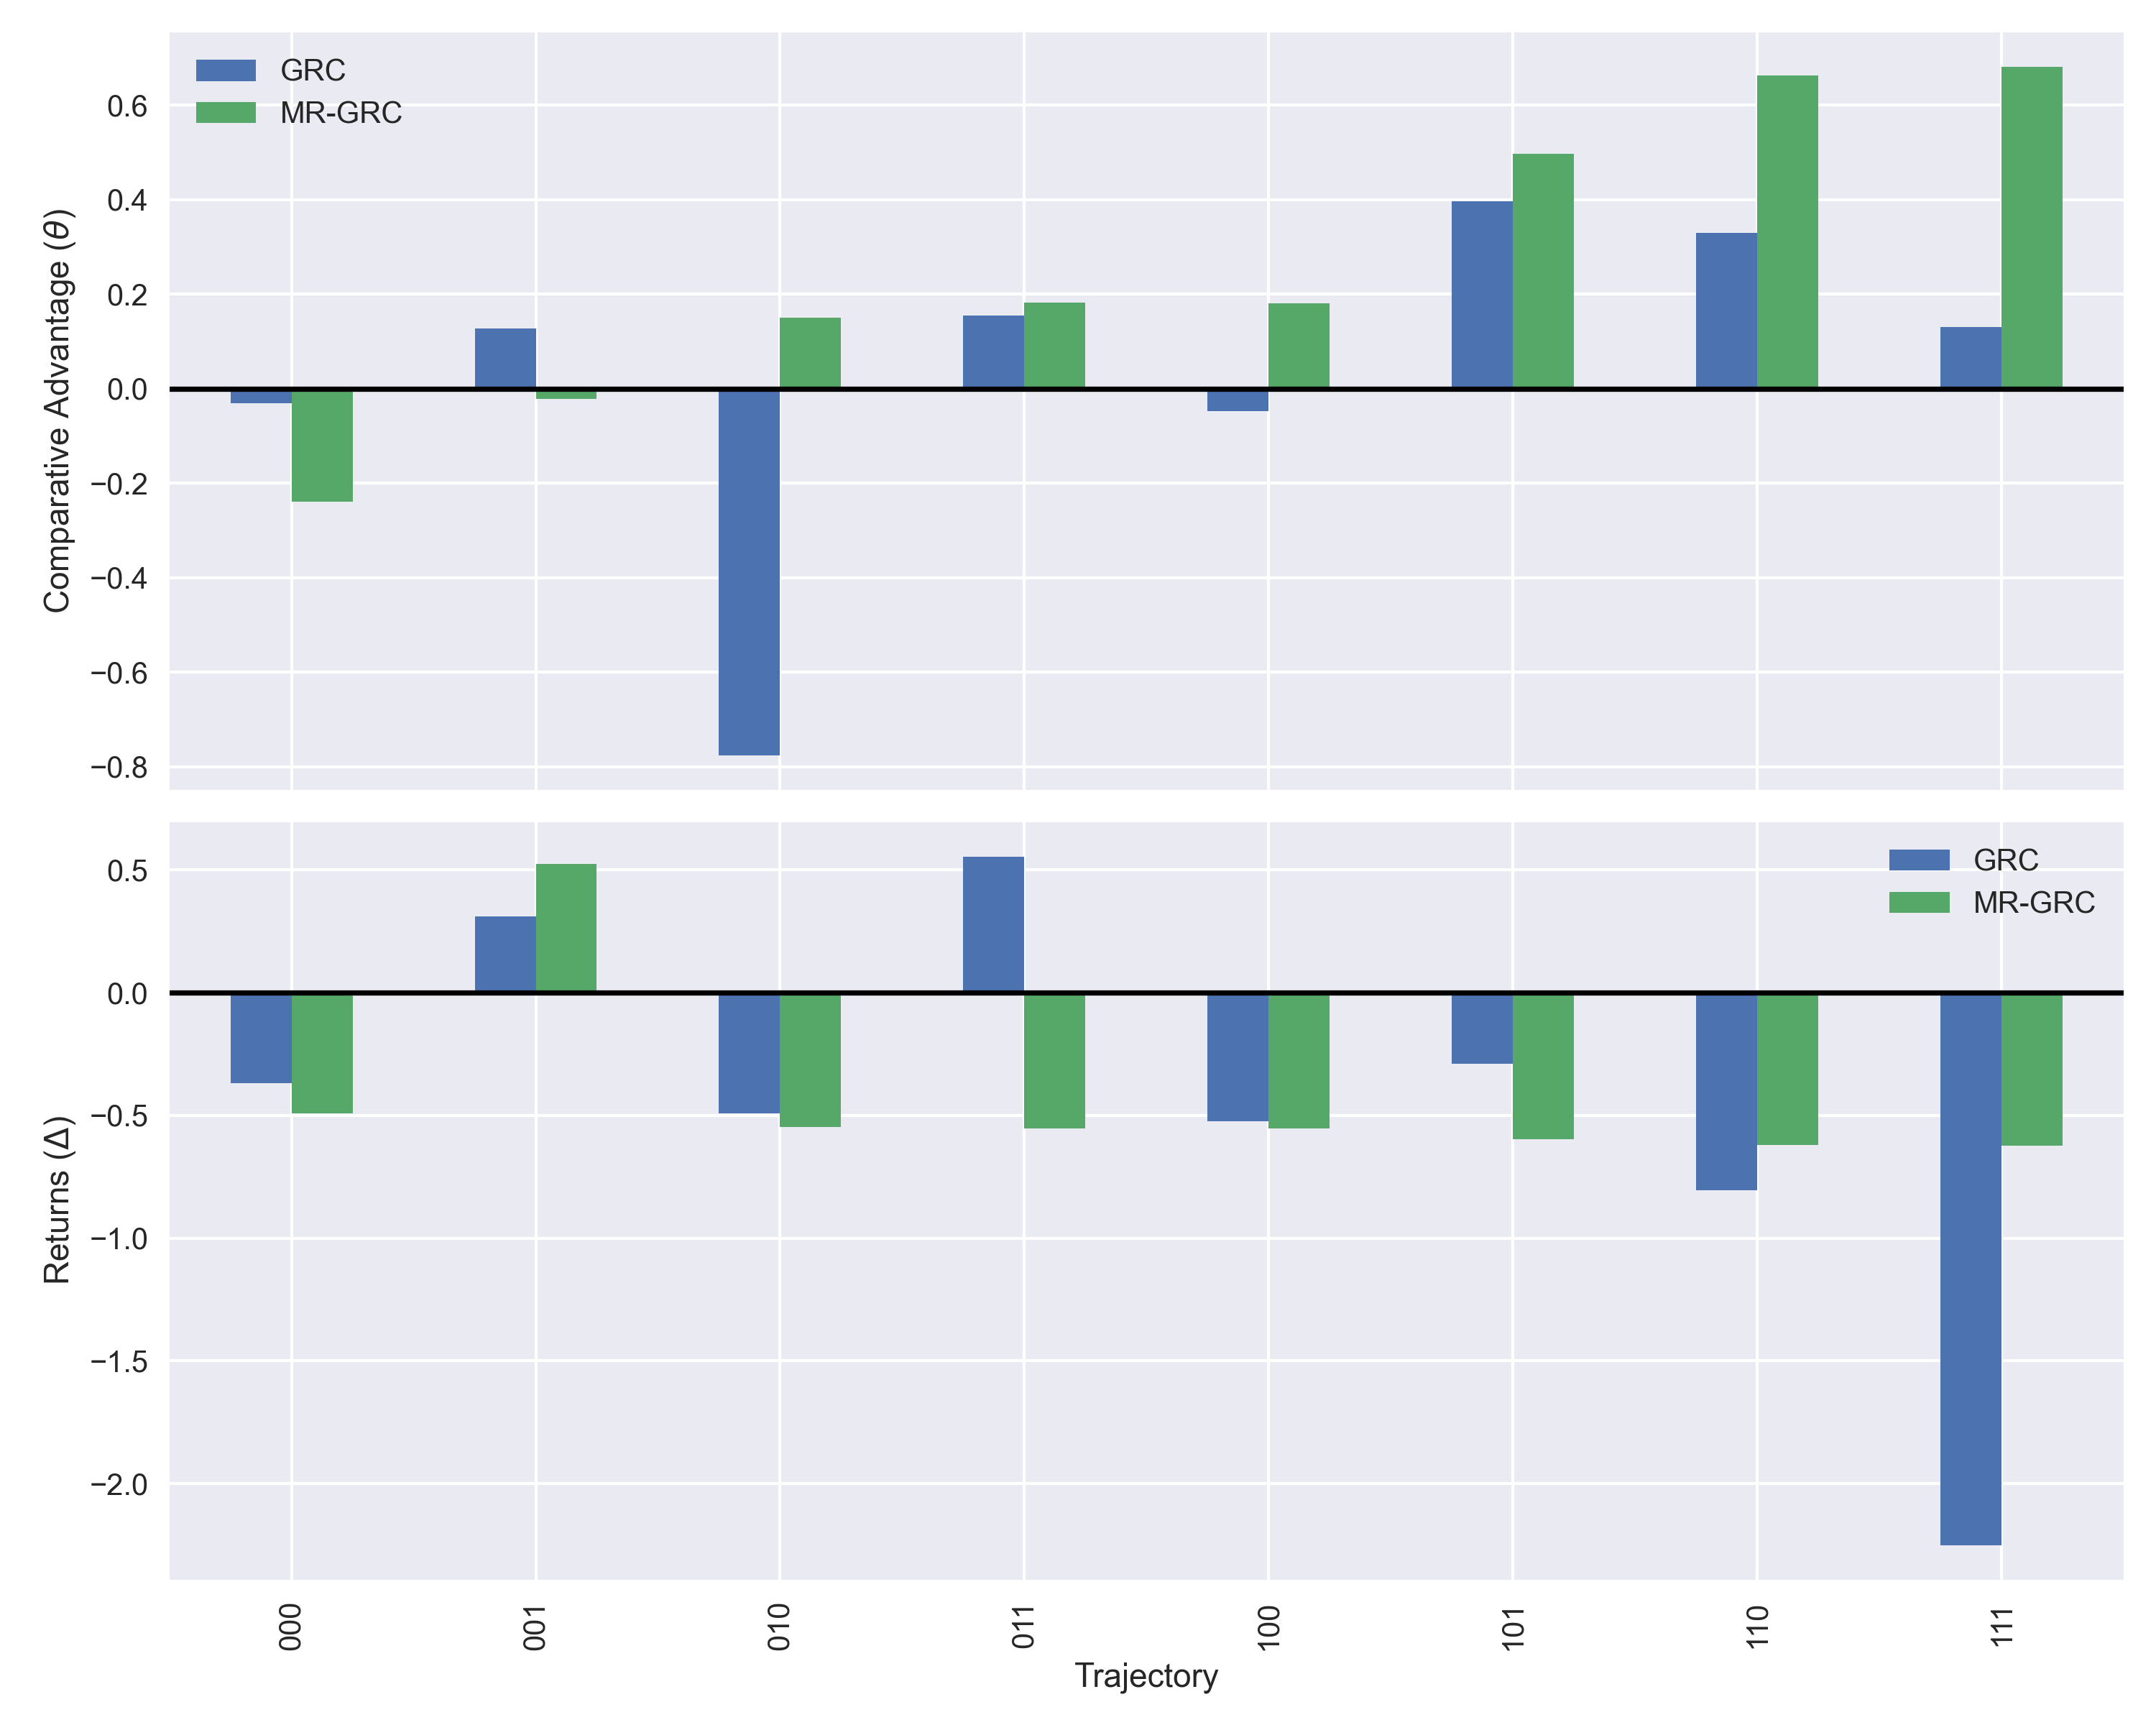
\includegraphics[scale=0.7]{results/figures/mr-theta.png}
    \caption{Comparative Advantage and Returns to Adoption: GRC and MR-GRC Results}
    \label{fig:mr-grc}
            \vspace*{-2em}
    \begin{table}[H]
        \centering
        \begin{tabular}{p{0.8\textwidth}} 
            \begin{tablenotes}
                  \small
                  \item Note: Figure shows GRC and MR-GRC results side-by-side. GRC results are identical as the ones from Figure \ref{fig:theta_delta_raw}. MR-GRC estimated using likelihood function in Eq. \ref{eq:mr-grc}. Misclassification defined using DNA purity data from the fourth wave of ESS. Log(Dry cropcuts) used as outcome. Top figure denotes comparative advantage for each trajectory. Bottom figure denotes returns to adoption for each trajectory.
            \end{tablenotes}
        \end{tabular}
    \end{table}
\end{figure}


\section{Discussion}\label{sec:disc}

To explain the patterns showcased in our results, we propose a simple conceptual model of genetic dilution. The evidence is consistent in that newly bred varieties do offer higher performance than traditional varieties, but such higher-yielding effects diminish over time, as newer generations of the improved seeds continue to be used. In contrast, traditional local varieties are well-adapted to the local agroecological conditions, and their reproduction over multiple generations shows consistent yields, assuming normal weather conditions. Depending on the specific improved varieties and the speed at which high-yielding effects diminish over time, there may be a threshold in time above which it may be more profitable to use a traditional variety than an improved one that has been around for too many generations (Figure \ref{fig:generations}). After such a threshold is reached, because improved varieties are more dependent on external inputs, at a constant rate of fertilizer application, the yields of the older-generation improved seeds would sharply decrease, so that local traditional varieties would return in higher productivity.


\begin{figure}
    \centering
    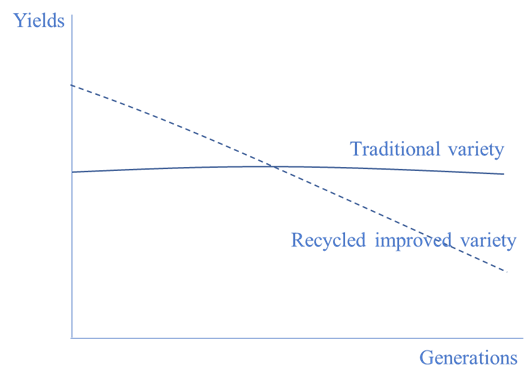
\includegraphics[scale=0.7]{results/figures/generations.png}
    \caption{Hypothetical yields for recycled and traditional varieties}
    \label{fig:generations}
\end{figure}

This depiction is certainly an over-simplification, as many crucial variables are taken as constant, such as seed costs, fertilizer application, water input use, weather conditions, and the specificities of the improved seeds (that would determine for example how resistant they are to drought conditions). Adding some of these features to a similar model, \cite{Bird2020-nt} propose a theoretical model where retained local traditional varieties are compared with two types of improved varieties: one that is non-locally adapted, and one bred for the specific local agro-climatic conditions. The authors postulate that while profits of both types of improved varieties increase with fertilizer application, profits of traditional varieties would decrease with fertilizer application, implying the existence of a threshold of fertilizer application below which it is more profitable to keep using traditional varieties. Non-locally adapted varieties are less profitable without complementary fertilizer application. Depending on how responsive to fertilizer both improved varieties are and on the costs of seeds, there may be a threshold of fertilizer application below which it is more profitable to use the locally adapted variety than the improved non-adapted one.

These findings may also hold for our case, especially taking into consideration the degree of genetic dilution and dispersion of recycled or older-generation improved varieties, which are not as yield responsive to fertilizer application. In addition to this, prior evidence also indicates that farmers sub-optimally allocate fertilizer in response to their mislead beliefs about the crop variety (\citealt{euler2022because}). Such wrong beliefs or misclassification has also been shown to be driven by misperception instead of misreporting (\citealt{wossen2022misperceiving}), which is also the case for the farmers in our sample. These findings suggest that the seemingly small to negative returns to adoption that we find through the GRC model are driven by both a lower response to fertilizers of the older-generation improved varieties, but also to farmers’ sub-optimal application of fertilizers (and possibly other inputs) due to misperception.

The suitability of the improved varieties to weather conditions and the weather conditions themselves are two additional factors that may further explain the seemingly negative comparative advantages to adopting the misperceived improved varieties. Even moderate droughts have been shown to decrease maize yields of non-drought tolerant varieties by 20\% (\citealt{paul2021heterogeneous}). Additionally, although our results confirm the positive returns to DTM adoption (consistent with \citealt{wossen2017measuring}), even the DTM varieties distributed in Ethiopia are only resistant to mild drought but would also fail like any other non-drought tolerant variety in case of severe droughts. 

In addition to these factors, we are solely evaluating the comparative advantages of improved varieties over maize yields, but further analysis on net returns would be crucial for this context. Obtaining a first-generation high-yielding variety or drought tolerant ones represents a significant investment for farmers that usually use traditional varieties (most of the sample). The fertilizer, irrigation and other complementary inputs necessary for the proper response of the improved varieties also represent a substantial investment. Because of this, our prior is that the findings from this study would be aggravated if the outcome variable was net returns instead of maize yields, but this remains an open question for future research.

\section{Conclusion}\label{sec:conclusion}

% - Why do we see that increasing purity leads to positive ATE
% - may be due to improved seed being more effective, but doesnt tell the whole story
% - barrier to purchasing the seed and associated inputs for poorer households, leading to reuse of seeds and being less effective

Our results showcase the challenges of identifying the returns to technology adoption when adoption is not promoted by a randomized control trial and when the characteristics of the technology (genetic purity) are not easily observed. We show that in the case of Ethiopia, the return to adoption of improved seed varieties appears to be negative, a result that we attempt to further understand by relying on seeds' DNA fingerprinting, obtained from the last round of the ESS. Accounting for the decay of the purity of the genetic material, its source and years upon release, reveals that those farmers that rely on newly bred improved varieties do show positive returns to adoption. Even without explicit DNA fingerprinting evidence, the GRC could show this trend with the comparative advantage results; returns are harmful to those with a high comparative advantage to adopt, but these returns are less negative with time. We speculate that this is due to the fact that new and more genetically pure hybrids are introduced, giving those that adopt higher yields than before.

But the fact that newly bred hybrids that have adapted well to local conditions outperform local varieties and older-generation improved seeds is not surprising given the large investments devoted to improve seed performance and the speed at which new high-yielding varieties are being developed. The results from the GRC model highlight how the fact that we imperfectly observe the use of newly improved seed and the degree of misclassification between self-reported improved seed and bred hybrids may partially explain why we do not see self-reported improved varieties grant positive returns to adoption. Reconciling these findings with the results from the Endogenous Switching Regression, we hypothesize that the negative returns to adoption mask a large heterogeneity in the returns to adoption. The switching results show that the positive returns to adoption only appear for those farmers using newly bred hybrid seeds provided directly by distributors. 

This result buttresses the fact that a large share of farmers are not able to obtain the promised greater yields from using improved varieties. This may be partially driven by the low-purchasing rates of newly bred varieties, but also by the under-use of critical inputs needed for the successful performance of hybrid seeds, such as fertilizers and irrigation, especially in drought-prone areas. More research is required in order to understand the barriers to adoption and input use. Such barriers may be crucial for households with less resources, which might be more likely to reuse improved seeds for many generations or buy older generations from other farmers at a cheaper price. The fact that all the sampled plots chosen for DNA fingerprinting showed purity percentages of 70 percent or higher is indicative that this might be the case, given the widespread dilution of improved genetic material. Such dispersion of improved genetic material also poses a challenge for the proper identification of the returns to adoption as it confounds the potential benefits of locally adapted hybrids, but also the benefits of traditional local varieties that may be better suited for certain agro-ecological conditions and for contexts of low-input use.  

Our results have far-reaching policy implications. The adoption and impact of genetically improved seeds are inherently heterogeneous. Our methodology incorporates this from the outset. Our findings highlight the wide distribution of the yield returns to adoption, partially explained by the low purchase of newly bred hybrids and the high dispersion of diluted improved genetic material over time. This points to the need for making policies oriented towards increasing the adoption of improved seeds and yields more inclusive, aiming at ensuring that improved varieties are not only available to purchase locally but also affordable. It is important to consider that improved varieties should also be locally adapted to specific agro-ecological conditions, such that their success is less dependent on external chemical inputs. Our findings also shed light on the need to better understand adaptation strategies when the conditions needed for the successful performance of improved seeds are lacking. These contexts include but are not limited to places subject to high weather variability or where low soil fertility is prevalent due to the use of excessive intensification and chemical input dependence. Resilience-enhancing strategies such as the use of drought-tolerant maize or irrigation use may be critical for such contexts, but their suitability for the heterogeneous pool of farmers needs to be better understood. 


%allowing us to investigate whether synergies between seed adoption and water conservation strategies interact; a key component to understanding how investment into such projects translates to economic returns. Moreover, our research informs on not only the adoption but also dis-adoption decisions of technologies as well. In this sense, we provide valuable information to policymakers on how to better target seed marketing or infrastructure to help agricultural households improve their livelihoods






% \textbf{Next steps}
% \begin{enumerate}
% add comments from slides
%     \item We shoudl try to frame our non-experimental results in the light of Suri's: With experimental data, one can test for thepresence of heterogeneous returns, but estimating the distribution of returns requires assump-tions about the underlying selection process, which is randomized away in such an experiment(see Heckman, Smith, and Clements (1997). he experimental and IV evidence appeared to indicate thatmaize growers in Kenya were leaving “money on the table” by not adopting hy-brid seed. However, the experiments and IV results reveal little else about thereturns. The framework of heterogeneous returns in this paper allows the es-timation of not just average returns, but also the distribution of returns acrossthe sample of farmers. I find strong evidence of heterogeneity in returns tohybrid maize, with comparative advantage playing an important role in the de-termination of yields and adoption decisions. Finally,the heterogeneity in returns to the hybrid technology, on the whole, suggestsquite rational and relatively unconstrained adoption of existing hybrid strains,in contrast to the evidence from the experimental and IV literatures
%     \item 
% \end{enumerate}




\bibliography{references}

\section{Appendix}

\subsection{GRC Results Table}

The results of the GRC regression are shown in Table \ref{tbl:unres}. The results for self-reported and cropcut yields are largely similar. There is some discrepancy in the self-reported yields in the first wave, and specifically with the $(1,0,0)$ trajectory. The return to adoption is negative for cropcuts, but positive for self-reported yields. The returns to adoption in many cases, are not statistically significant, or they are negative. Only in the case of the trajectory $(0,0,1)$: those that adopted in the second and third waves, is there a large, statistically significant effect. 

In order to calculate comparative advantage, there must be evidence for the LCA being satisfied. The lower panel of  Table \ref{tbl:unres} shows the results for the weak identification test for $\phi$, including each trajectory on its own and a joint test. We can see here that for the case of cropcuts with controls, there is a confidence interval for the joint test of $\phi$, giving evidence to the fact that the LCA is satisfied most prominently in that case. For the aggregations for this paper, then, we will use that specification.

\begin{landscape}
{
\def\sym#1{\ifmmode^{#1}\else\(^{#1}\)\fi}
\begin{tabular}{l*{6}{c}}
\hline\hline
          &\multicolumn{1}{c}{(1)}&\multicolumn{1}{c}{(2)}&\multicolumn{1}{c}{(3)}&\multicolumn{1}{c}{(4)}&\multicolumn{1}{c}{(5)}&\multicolumn{1}{c}{(6)}\\
          &\multicolumn{1}{c}{Log Dry Cropcuts}&\multicolumn{1}{c}{Log Dry Cropcuts}&\multicolumn{1}{c}{Log Dry Cropcuts}&\multicolumn{1}{c}{Log Self-Report}&\multicolumn{1}{c}{Log Self-Report}&\multicolumn{1}{c}{Log Self-Report}\\
\hline
$\mu_{000}$&    6.350\sym{***}&    6.387\sym{***}&    6.346\sym{***}&    6.587\sym{***}&    6.468\sym{***}&    6.444\sym{***}\\
          & (0.0373)         &  (0.140)         &  (0.165)         & (0.0310)         &  (0.109)         &  (0.134)         \\
$\mu_{001}$&    6.246\sym{***}&    6.468\sym{***}&    6.431\sym{***}&    6.659\sym{***}&    6.620\sym{***}&    6.622\sym{***}\\
          &  (0.121)         &  (0.181)         &  (0.197)         &  (0.103)         &  (0.138)         &  (0.159)         \\
$\mu_{010}$&    6.405\sym{***}&    6.478\sym{***}&    6.448\sym{***}&    6.942\sym{***}&    6.844\sym{***}&    6.835\sym{***}\\
          &  (0.151)         &  (0.219)         &  (0.238)         &  (0.118)         &  (0.163)         &  (0.186)         \\
$\mu_{011}$&    5.518\sym{***}&    5.649\sym{***}&    5.617\sym{***}&    5.968\sym{***}&    5.911\sym{***}&    5.930\sym{***}\\
          &  (0.207)         &  (0.226)         &  (0.240)         &  (0.363)         &  (0.377)         &  (0.393)         \\
$\mu_{100}$&    6.479\sym{***}&    6.584\sym{***}&    6.545\sym{***}&    6.759\sym{***}&    6.698\sym{***}&    6.685\sym{***}\\
          &  (0.145)         &  (0.207)         &  (0.226)         &  (0.114)         &  (0.154)         &  (0.173)         \\
$\mu_{101}$&    6.466\sym{***}&    6.565\sym{***}&    6.527\sym{***}&    7.011\sym{***}&    6.850\sym{***}&    6.838\sym{***}\\
          &  (0.193)         &  (0.243)         &  (0.263)         &  (0.166)         &  (0.196)         &  (0.213)         \\
$\mu_{110}$&    6.908\sym{***}&    6.931\sym{***}&    6.898\sym{***}&    7.120\sym{***}&    7.000\sym{***}&    6.983\sym{***}\\
          &  (0.277)         &  (0.306)         &  (0.320)         &  (0.124)         &  (0.161)         &  (0.180)         \\
$\Delta_{001}$&    0.634\sym{***}&    0.469\sym{*}  &   -6.213\sym{***}&    0.209         &    0.113         &   -7.050\sym{***}\\
          &  (0.241)         &  (0.251)         &  (0.296)         &  (0.152)         &  (0.146)         &  (0.202)         \\
$\Delta_{010}$&   0.0398         &   0.0438         &   -6.507\sym{***}&   0.0531         & -0.00684         &   -7.174\sym{***}\\
          &  (0.319)         &  (0.344)         &  (0.403)         &  (0.138)         &  (0.137)         &  (0.207)         \\
$\Delta_{011}$&    1.308\sym{***}&    1.214\sym{***}&   -5.439\sym{***}&    1.241\sym{***}&    1.179\sym{***}&   -6.002\sym{***}\\
          &  (0.250)         &  (0.236)         &  (0.284)         &  (0.380)         &  (0.374)         &  (0.412)         \\
$\Delta_{100}$&   -0.699\sym{***}&   -0.599\sym{***}&   -7.360\sym{***}&    0.718\sym{***}&    0.640\sym{***}&   -6.484\sym{***}\\
          &  (0.252)         &  (0.195)         &  (0.266)         &  (0.136)         &  (0.149)         &  (0.205)         \\
$\Delta_{101}$&    0.112         &    0.270         &   -6.340\sym{***}&    0.157         &    0.216         &   -6.984\sym{***}\\
          &  (0.321)         &  (0.374)         &  (0.395)         &  (0.262)         &  (0.257)         &  (0.299)         \\
$\Delta_{110}$&   -0.302         &   -0.177         &   -6.926\sym{***}&   -0.421\sym{***}&   -0.379\sym{**} &   -7.497\sym{***}\\
          &  (0.304)         &  (0.297)         &  (0.345)         &  (0.158)         &  (0.173)         &  (0.233)         \\
8.trajectory#1.impmaize&    6.606\sym{***}&    6.704\sym{***}&        0         &    7.256\sym{***}&    7.180\sym{***}&        0         \\
          & (0.0707)         &  (0.153)         &      (.)         & (0.0539)         &  (0.124)         &      (.)         \\
\hline
Observations&      984         &      974         &      974         &     2320         &     2289         &     2289         \\
Controls  &       No         &      Yes         &      Yes         &       No         &      Yes         &      Yes         \\
Interact w/ Hybrid&       No         &       No         &      Yes         &       No         &       No         &      Yes         \\
\hline\hline
\multicolumn{7}{l}{\footnotesize Standard errors in parentheses}\\
\multicolumn{7}{l}{\footnotesize \sym{*} \(p<0.10\), \sym{**} \(p<0.05\), \sym{***} \(p<0.01\)}\\
\end{tabular}
}

\end{landscape}

\end{document}